\documentclass{cumcmthesis1}
% \documentclass[withoutpreface,bwprint]{cumcmthesis} %去掉封面与编号页,电子版提交的时候使用。

\lstset{
  language=Matlab,                   % 设置语言为MATLAB
  basicstyle=\ttfamily\footnotesize, % MATLAB 使用等宽字体,设置较小字体
  keywordstyle=\color[rgb]{0,0,1},   % 关键字的颜色(蓝色)
  commentstyle=\color[rgb]{0.13,0.54,0.13}\itshape, % 注释颜色(绿色,斜体)
  stringstyle=\color[rgb]{0.6,0.1,0.1}, % 字符串颜色(深红色)
  numbers=left,                      % 显示行号
  numberstyle=\tiny\color{gray},     % 行号样式
  stepnumber=1,                      % 行号的步进
  numbersep=10pt,                    % 行号与代码间的距离
  backgroundcolor=\color{white},     % 背景颜色保持白色
  frame=single,                      % 代码块的边框
  tabsize=4,                         % MATLAB 中的默认 Tab 缩进
  captionpos=t,                      % 标题位置在上方
  breaklines=true,                   % 允许自动换行
  breakatwhitespace=false,           % 仅在空白处换行
  showspaces=false,                  % 不显示空格符号
  showstringspaces=false,            % 不显示字符串中的空格符号
  showtabs=false,                    % 不显示Tab符号
  morekeywords={matlab_specific_keyword}, % 可自定义其他MATLAB关键字
}
\usepackage[framemethod=TikZ]{mdframed}
\usepackage{url}   % 网页链接
\usepackage{subcaption} % 子标题
\usepackage{float}
\title{“板凳龙”模型实时仿真模拟}
\tihao{A}
\baominghao{4321}
\schoolname{中山大学}
\membera{张洋 }
\memberb{邓俊辉 }
\memberc{殷润轩 }
\supervisor{ }
\yearinput{2024}
\monthinput{09}
\dayinput{22}

\begin{document}

 \maketitle
 \begin{abstract}
 本文针对“板凳龙”运动问题,结合物理学相关规律,建立一套实时仿真模拟的“板凳龙”物理模型。通过近似圆弧法、叉积法、非线性动态规划,实时仿真模拟等方法进行计算机求解。在给定的不同的螺距、“板凳龙”运动方式、位置、速度等多种情况下,解决了“板凳龙”各节龙身位置、速度与调头转向等多个运动学问题。
 \par
 对于给定螺距、前把手运动速度、龙头初始位置的各节龙身运动位置速度求解问题,将该运动过程划分为龙头运动过程与各节龙身运动过程,分别进行建模。龙头运动位置,通过建立极坐标系下螺线的轨迹方程、龙头把手极坐标关于时间的解析表达式、将瞬时的螺旋运动等效为圆弧运动等方法,从而计算出龙头的实时位置坐标。再利用速度差分法,将一小段微小时间内平均速度等效为瞬时速度的方法得到各把手实时速度表达式。
 \par
 对于给定螺距、龙头初始位置的各节板凳碰撞问题,首先通过证明三个断言,给出了简化计算的理论依据。我们将碰撞问题转化为了龙头左前边界点与其后续18节板凳矩形位置关系问题,通过叉积法判断矩形与点的位置关系。结合问题1的实时仿真模拟,解得龙头在到达螺旋线中心前已和第八节龙身板凳相碰撞,该时刻为413.36s。
 \par
 对于逆时针盘出、发生调头情况的龙头运动求解问题,可以将该问题转化成在不同螺距下求解碰撞点螺旋半径的问题。通过不断减小螺距步长,使得碰撞点螺旋半径不断接近调头半径。循环调用求解问题2所使用的算法,直至螺距到达最优值0.45m。
 \par
为了求出在掉头区域内完成调头的最短路程问题,我们首先分析在严格限制半径比值1:2情况下的最优调头路程,通过对其自由度的分析可知这是个非线性规划问题,只有唯一解。为了
 \par
对于盘出螺线与盘入螺线关于螺线中心呈中心对称、各龙身把手速度均不超过2m/s的“板凳”运动问题,处理方法与问题四是相类似的。将第四问求出的横纵坐标与时间相关的表达式,转化为以时间与速度为变量的表达式。已知所有板凳的速度上限为2m/s,则可从$v_{head}$=1m/s开始,以dv步长不断增大,依次对每一秒遍历。经过多次计算,龙头最大行进速度为1.10m/s。
 

\keywords{\quad  仿真模拟\quad   近似圆弧法\quad 差分法 \quad 非线性规划 \quad 叉积法 \quad 循环迭代 \quad 几何法  \quad矩阵计算 \quad 算法设计}
\end{abstract}
\section{问题背景与重述}
\subsection{问题背景}
本文所研究的问题基于“板凳龙”这一独特的文化活动。板凳龙, 是起源于河洛地区的传统民俗活动之一,普遍存在于我国南方各省市的年度盛大活动。这一元宵节习俗已有几个世纪。其中福建是当地人迎神、祈福的一项民俗活动,蕴含着深厚的地域文化。2008年春节,中国福建省三明市大田县的“板凳龙”被列为国家级非物质文化遗产推荐项目。板凳龙相传源于汉代,由“舞龙求雨 ”的宗教活动演变而来。而大田的板凳龙的习俗据闻由八姓入闽时期中原的先民所带来,如今,大田板凳龙已成为远近闻名传统习俗。村民们把一节节的板凳钻孔连接,一户一节,组成板凳长龙,可达两百多米长,非常壮观。当地的居民将几十条乃至上百条的板凳首尾相连,形成蜿蜒曲折的“盘龙”,整体呈圆盘状。\par
本文所研究的问题正是基于这一文化活动给出的具体化数学问题。问题要求我们对一条整体为螺线结构的“盘龙”进行分析,从实际的物理现象中抽离出数学物理模型,建立方程并求解。
题目给出了每条板凳的结构与相关数据。本文结合实际,建立数学模型,对以下问题进行了探讨与求解。\par
\subsection{问题要求}

\par 
\textbf{问题1:} 问题1要求我们建立合理的数学模型,用来描述舞龙队沿螺距为55Lm的等螺距逆时针盘入的全过程。前把手的行进速度恒定为1m/s,问题要求我们计算从初始时刻到300秒为止,每一秒龙头身和龙尾各前把手及龙尾后把手的位置和速度。问题要求我们将结果保存到指定的命名文件中。针对该问题,我们结合物理定律与仿真模拟,在极坐标系下建立了螺线方程,从而确定各处的位置与速度。该过程中我们将螺旋运动近似看作圆周运动,而螺旋线并非严格的圆弧,故而必然导致几度或分秒级的误差,随后我们引入误差度 \text{$\eta$}与修正系数 \text{$\alpha$}得出了修正后的极坐标方程解析表达式。对于后续龙身把手位置,我们分别采用余弦法与近似圆弧法求解。针对把手速度,我们采用差分法求解。
\par
\textbf{问题2:}在问题1的基础上,本问题要求深入剖析终止时刻所对应的物理意义,并将其作为约束条件,确定舞龙队盘入的终止时刻。换言之,就是确定出即将发生碰撞而受迫无法再继续盘入的时间。我们需要计算并给出此时舞龙队的位置,并将结果保存到指定的文件中。针对该问题,我们将板凳的面近似为一个长矩形,因此需要给出一个点是否位于另一个矩形内部的判断依据。引入叉积法,用于判断点是否在矩形内,若在矩形外,即满足保持运动的条件,则增加时间步长继续求解;反之,则证明已经发生过碰撞,发生碰撞的时刻即为终止时间。我们找出一个显然还未相撞的时间点,并以该时间点为起点,逐步迭代确定终止时间。
\par
\textbf{问题3:}问题3引入了一个全新的概念——“调头空间”,即以螺线中心为圆心、直径为9m的圆形区域。问题要求我们确定最小的螺距,使得龙头前把手能够沿着相应的螺线盘入到空间的边界,同时必须保证板凳之间不发生碰撞。与问题2相似,当螺距最小时,龙头左前方把手刚好在调头时与某一部分龙身发生碰撞。此时,我们可以从0开始逐渐增大螺距,找出刚好满足题意时的螺距,此时便确定了最小的螺距。
\par
\textbf{问题4:}问题4区别于前3个问题,设定了新的盘入和盘出条件。盘入螺线的螺距为1.7m,盘螺线与盘入螺线关于螺线中心呈中心对称。在问题3设定的调头空间内,舞龙要完成调头。调头路径是由两段圆弧相切连接而成的S形曲线,其中前一段圆的半径是后一段的2倍,且与盘入、盘出螺线均相切。问题要求我们探讨是否可以通过圆弧来缩短调头曲线,同时保持各部分相切。还需要计算从-100秒到100秒内每秒舞龙队的位置和速度,并在论文中给出特定时间点的数据。题目给出了前一段圆的半径是后一段的2倍时的条件,要求我们改变半径比,从而使调头曲线变短。很自然地,我们想到去求得调头曲线的最小值。因为此时调头曲线必然是变短的,很明显符合题意。详细的求解过程见下文的建模与求解。
\par
\textbf{问题5:} 基于问题4设定的路径,问题5要求确定龙头的最大行进速度,使得舞龙队各把手的速度均不超过2m/s。第四问求出的横纵坐标与时间相关的表达式,转化为以时间与速度为变量的表达式。由题意可知,所有板凳的速度均不超过2m/s,则可从$v_{head}$=1m/s开始,以dv步长不断增大,遍历-100s到100s的每一秒。当某一部分速度恰好达到2m/s时,取此时龙头的速度为最大速度。




\section{问题分析}
\subsection{\textbf{问题1}:求解“板凳龙”各把手实时坐标和速度}
\par
问题一要求我们建立模型来计算“板凳龙”各个把手在螺线上的实时坐标和速度。首先,我们需要将具体的运动抽象成方便理解与运算的物理模型。分析了具体情境之后,我们发现,由于问题1侧重于各部分的运动,尚未考虑不同板凳之间的相互碰撞问题,因此我们可以将这223节“板凳龙”的运动质点化,从而利用题干信息求解结果。\par
根据螺线的性质,我们选择在极坐标中建立螺线的轨迹方程。即抽象成连接有224个把手的细杆刚体运动模型,其中每个把手均位于螺线上,各把手间欧式距离由实际意义保持恒定。考虑题干中所给的龙头信息,由于龙头线速度恒定为1m/s,根据角速度微分表达式和瞬时表达式,结合龙头初始值可以建立微分方程模型,等式两边定积分可求出龙头的角位移随时间变化关系表达式,再根据轨迹方程和平面坐标投影关系便得到龙头的实时坐标。
\par
我们发现由于各把手与其上一个把手用“板凳”刚性连接,故它们的运动学特征存在关联。因此,我们可以建立循环迭代模型,只要前一个把手的运动学参数已知,就能在一次循环节中求得下一个把手的相关运动学参数。在处理相邻的把手时(即一个循环节中),由于螺线在一个微小角位移变化下其半径几乎不变,故而可以将相邻把手间的螺线等效为一小段微小的圆弧处理,且因连接把手的有效板凳长相对于半径为一个小量,因而可以进一步以直代曲,直接将有效板凳长度当做圆弧长来计算两把手对应的角位移差值,从而顺利得到了下一个把手的角位移大小,相应地,就不难求出其位置参数。在下面的章节中,我们还将介绍一种使用三角余弦定理结合超越方程数值解的迭代方法,并比较两种方法的误差程度,并且说明选择前者做法的理由。
由于每个把手的实时位置坐标已知,接下来我们可以通过瞬时速度的近似定义,即
一段微小时间内的位移除以时间长度来求出具体的速度参数。
\subsection{\textbf{问题2}:}
问题二要求我们建立模型考虑“板凳龙”盘入的终止时刻。首先,我们需要明确,“板凳龙”的盘入终止可以分为两种情况。第一种为舞龙队龙头到达螺线的中心,无法再继续前进,则盘入自然终止;第二种为,早在龙头到达螺线的中心之前,舞龙队的龙头与其中一节龙身之间就已经发生了碰撞,则盘入的过程必然终止。
我们需要将“碰撞”情况用数学的语言去区分和描述。因此,我们将板凳面等效为一个长矩形。故而,给出一个点是否位于另一个矩形内部的判断依据是必要的。我们引入叉积法来解决这个问题。该方法的详细步骤可分为:确定矩形的顶点、计算点到矩形各边的叉积以及判断点关于矩形的位置。若存在某一时刻,使得一个板凳的某个边界点出现在另一个矩形内部,则说明在该时刻之前,已经发生了碰撞,则运动必然终止。若这个时刻不存在,则龙头顺利到达终点,运动自然终止。
我们应用MATLAB语言验证上述模型与假设,在逐步迭代的过程中,发现左前把手与第八节龙身在某一时刻发生了碰撞,运动也随之而终止。关于这一过程,详细的求解步骤将在下文中展示出来。
\subsection{\textbf{问题3}:}
和问题2相似,问题3同样要求我们考虑碰撞条件。首先,我们需要明确,圆形的“调头空间”基于龙头先到达中心并转向的假设。因此,我们必须先筛选出满足龙头到达中心的时刻,才能进行后续操作。
我们需要考虑“调头空间”所对应的物理意义。可以知道,“调头空间”越小,龙头前把手调头后与龙身发生碰撞的时刻越早。因此,我们可以通过发生碰撞的时刻,反向进一步确定“调头空间”的最小值。
我们从0开始,不断增大“调头空间”的值,直到龙头前把手调头时刚好与龙身发生碰撞。此时,我们便成功确定了“调头空间”的最小值。
\subsection{\textbf{问题4}:}
问题4给出了一套全新的框架,首先,我们需要读懂题意。可以明确的是,由盘入曲线中心与盘出曲线中心关于圆心对称可知,它们的连线必然经过圆心。另外,在盘入曲线与圆弧、盘出曲线与圆弧相交的两点,是相切的,即斜率相同,更进一步的说,关于时间的变化率相同。题目还给出大圆弧的半径为小圆弧的两倍。
其次,当半径比固定时,盘入曲线的横纵坐标、盘出曲线的横纵坐标以及半径比五个变量对应五个已知条件,此时有关圆弧与螺旋线的所有条件都是逻辑自洽的。然而,题目要求我们改变半径比,即五个变量对应了四个已知条件。可以看出,调头曲线的长度可以用半径与角度求得。因此,问题4变成了我们所熟悉的非线性规划问题。
最后,我们将约束条件改写为数学公式,目标函数正是题目要求我们计算的调头曲线,带入MATLAB求解即可得出答案。至此,我们将减小调头曲线的目标修正为求解调头曲线最小值的工作全部完成。
\par
问题4的第二问与第一问相似,我们可以解出调头曲线的数学表达式。首先,我们需要对舞龙队的运动作分类,由于约束条件的存在,所有龙身的运动都可以由龙头的运动情况推出。因此,我们直接对龙头的运动分情况讨论即可。
其次,龙头的运动状况可以分为在第一个圆弧上运动、在第二个圆弧上运动以及盘出曲线。值得注意的是,盘出曲线视为与盘入曲线关于螺旋线中心对称。因此只需考虑盘入曲线的结果并取相反数便可。
利用约束条件求出所有龙身板凳的运动状况,将其列入表格当中。
\subsection{\textbf{问题5}:}
问题5基于问题4,令原本固定的速度v也成为变量。首先,我们需要明确,满足什么条件时,龙头达到了最大行进速度。题干中提出了要求,所有板凳的速度均不可超过2m/s。因此,不难判断,当板凳龙的某一部分速度恰好达到2m/s时,此时龙头将达到最大行进速度。
其次,我们需要将约束条件转化为数学表达式,若存在$v_(t,v_{head})>2m/s$,那么取最大值$v_{max} = v_{head}-dv$。
结合物理知识,运用模拟仿真技术,从$v_{head}=1m/s$开始,以$dv$步长不断增大,遍历-100s到100s的每一秒,顺利得出龙头的最大行进速度。




\section{模型假设}
\par
以下是我们在模型建立与求解时为了尽可能简便计算所作出的合理假设:
\begin{enumerate}
    \item 一开始所有“板凳龙”的把手都已处于该螺旋线上。即在0时刻,不仅仅龙头严格位于
    \item “板凳龙”可以被看作是一个由224个离散把手刚性连接的系统,每个把手代表一个板凳把手中心,这样我们可以忽略板凳的形变与内部结构,有助于模型的简化。
    \item “板凳龙”龙头的速度被设定为恒定值(1m/s),每个把手严格按照路径运动,如均位于螺线或者圆弧线上。这种假设有助于使得运动更加理想化,尽管在现实中这种运动很难严格按照指定的速度与路线。
    \item 板凳之间的连接完全光滑,忽略实际生活中存在的摩擦力,把手振动问题。在实际问题中,我们还需要考虑由摩擦等因素带来的能量损耗。
    \item 在研究板凳间碰撞问题时,假设所有的板凳全部在同一平面内,尽管至少相邻的板凳连接一定会存在高度差。基于这种假设,我们只需要考虑平面内的碰撞,忽略三维运动和碰撞。
    \item 在现实中,板凳的运动方程,包括其位置与速度参数一定是连续可微的,即可作图为一张连续光滑的曲线。在模型的建立与求解过程中,我们只能将时间假设为离散的分立数值,但是可以不断减小时间的步长,从而增强其连续性。
\end{enumerate}
\newpage
\section{符号说明}
\par 以下是建立模型时用到的主要符号及其说明

\begin{table}[h!]
    \centering
    % 使用tabularx环境,并指定总宽度为\textwidth
    \begin{tabularx}{\textwidth}{c|X}
    \toprule
    \textbf{符号} & \textbf{含义说明} \\
    \midrule
    $L_{head}$ & 龙头长度(m) \\
    $L_{body}$ & 龙身长度(m) \\
    $d$ & 孔中心距离最近的板头距离(m) \\
    $L_{eff1}$ & 龙头有效连接长度(m),这里为$L_{head}-2d$ \\
    $L_{eff2}$ & 龙身有效连接长度,这里为$L_{body}-2d$ \\
    $v_{head}$ &  龙头把手线速度(1m/s)\\
    $w$ & 板宽(m) \\
    $p$ & 螺距(m) \\
    $b$ & 螺线系数,这里$b=p/2 \pi$ \\
    $\theta_i$ & 第$i$个把手(第$i-1$段龙身的前把手)的角位移(rad/s)\\
    $r_i$ & 第$i$个把手的螺线半径(m) \\
    $\omega$ &角速度 (m/s)\\
    $(x_i, y_i)$ & 第$i$个把手对应的横纵坐标 (m)\\
    $(v_{ix}, v_{iy}, v_{i})$ & 第$i$个把手对应的三个速度参量(m/s) \\
    $ \begin{bmatrix}
    (x_{ifl}, y_{ifl}) & (x_{ifr}, y_{ifr}) \\
    (x_{ibl}, y_{ibl}) & (x_{ibr}, y_{ibr})
    \end{bmatrix} $ & 第$i$个把手所处板凳四个边界点坐标矩阵 \\
    $R $ & 掉头区域半径 (m)\\
    $\gamma$ & 螺旋线与圆切线方向的夹角(rad)\\
    $\eta$ & 速度误差\\
    $\alpha$ & 速度修正函数\\
    $S $ & 调头曲线长度(m)\\
    $r_1, r_2$ &  两条圆弧的半径(m)\\
    $\theta_1 , \theta_2$ & 两条圆弧对应的夹角(rad)\\
    $t_0$ & 龙头进入第一条圆弧线的时刻(s)\\
    $t_{n1}$ & 龙头离开第一条圆弧线的时刻(s)\\
    $t_{n2}$ & 龙头离开第二条圆弧线的时刻(s)\\
    \bottomrule
    \end{tabularx}
\end{table}



\section{模型的建立与求解}
\subsection{\textbf{问题1}模型建立与求解}
\par
问题一要求求解任意t时刻所有把手的位置与速度参数。根据各个把手刚性相连的特点,只要已知龙头的运动参数,就可以通过循环迭代将龙头后连接的所有把手的运动参数求出。
同时,应尽可能提高提高相关龙头运动参数的精确度,否则通过循环迭代求解出的其他后续把手必然也会存在较大误差。
\subsubsection{\textbf{问题1}龙头位置求解}
\par
首先建立极坐标系下螺线的轨迹方程,相应地得出以$t$为变量的螺旋线上龙头把手的运动方程:
\begin{equation}
r(\theta)=\frac{11 \theta}{40 \pi}
\end{equation}
\begin{equation}
    r(t)=\frac{11 \theta(t)}{40 \pi} 
\end{equation}
\par
下面建立微分方程模型进而求解出不同时刻$t$下龙头把手极坐标的解析表达式。分别展开角速度
$\omega (t)$的微分表达式和瞬时决定式,并使其相等从而得到一个微分方程。
\begin{equation}
    \text{由}\vec{v}=\vec{\omega} \times \vec{r} \quad \text{有}       \frac{v(t)}{r(t)}=-\omega (t)=-\frac{d \theta}{dt}
\end{equation}
\par
其中,根据题目所给条件,龙头把手从初始坐标$(8.8,32\pi)$开始顺时针盘入中心,故其角位移$\theta(t)$
逐渐减小,因此$\omega (t)$前添符号。下面对(3)式两边求定积分:
\begin{equation}
\int_{32 \pi}^{\theta}  \theta \,d\theta =-\frac{40 \pi}{11}\int_{0}^{t}  \,dt 
\end{equation}

得到龙头把手中心极坐标表达式:
\begin{align}
    \begin{cases}
        \theta(t)=\sqrt{(32\pi)^2-80\pi t / 11}\\
        r(t)=11 \theta(t)/40 \pi 
    \end{cases}
\end{align}
\par
相应地,在平面直角坐标系投影螺旋半径可以求出龙头把手关于时间$t$的解析表达式:
\begin{align}
    \begin{cases}
        x(t) = r(t) \cos \theta(t)\\
        y(t) = r(t) \sin \theta(t)\\
    \end{cases}
\end{align}
\par
为了进一步求出当前时刻的横纵方向分速度$v_{1x}$和$v_{1y}$,可以通过链式法则对上面的式子进行求导:
\begin{align}
    \begin{cases}
        v_{1x}(t) = \cos\theta(t) \cdot \frac{dr(t)}{dt} - r(t) \sin\theta(t) \cdot \frac{d\theta(t)}{dt} \\
        v_{1y}(t)= \sin\theta(t) \cdot \frac{dr(t)}{dt} + r(t) \cos\theta(t) \cdot \frac{d\theta(t)}{dt}
    \end{cases}
\end{align}
\par
其中:
\begin{align}
    \begin{cases}
        \frac{dr(t)}{dt} = -\frac{1}{\sqrt{(32\pi)^2 - \frac{80}{11}\pi t}}\\
        \frac{d\theta(t)}{dt} = -\frac{4\pi}{110 \sqrt{(32\pi)^2 - \frac{80}{11}\pi t}}
    \end{cases}
\end{align}
\par
由于把手沿着螺旋线运动,而螺旋线并不是一个严格的圆弧,这就导致了其线速度和螺旋矢径之间的夹角并不是一个严格的直角,必然存在几度或分秒级别的误差。
在(3)式中,我们是将这样的螺旋运动在各个时刻下的状态与其在同样半径的圆弧运动作了一步近似。因此在(3)式中,可以忽略
径向速度$v_r(t)$,并直接将圆周运动的切向速度$v_\theta(t)$等效为螺旋运动的线速度$v(t)$。
\begin{figure}
    \caption{螺旋运动和近似圆周运动夹角}
    \centering    
    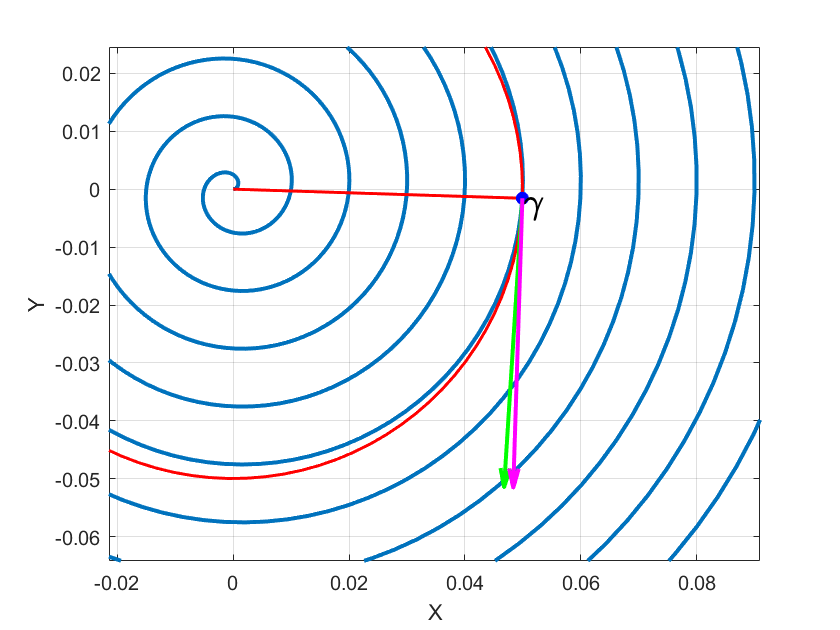
\includegraphics[width=0.68\linewidth]{drawing_t1_1.png}
\end{figure}
\par
假设任意一点处螺旋线的切线方向和相同半径圆弧切线方向夹角
(即图中紫线和绿线之间的夹角)为$ \gamma $(见图1)。我们可以通过先前的物理量推出$ \gamma $与$ \theta $之前的关系式。为了拟合得到更好的数据,我们考虑螺线与圆弧之间的运动关系并用数学关系来定量表示。我们需要用到切向矢量来表达这两个量,等价关系可由以下式子导出:
\begin{align}
    \begin{cases}
    \vec{a}  = ( cos{\theta}-{\theta}sin{\theta}, sin{\theta}+ {\theta}cos{\theta}  )\\
    \vec{b}  = (cos{\theta},  sin{\theta}   )\\
    cos{\gamma}  =\vec{a}\cdot\vec{b} /|\vec{a}| |\vec{b}| 
    \end{cases}
\end{align}
其中$\vec{a}$为螺旋线的切向矢量,$\vec{b}$为圆周的切向矢量,联立并求解上述式子,有以下关系:
\begin{equation}
    cos{\gamma} = \frac{1}{1+{\theta}^2}
\end{equation}
对式子变形,有:
\begin{equation}
    \gamma = arccos{\frac{1}{1+{\theta}^2}}
\end{equation}
不难看出,在角位移较小时,$\gamma$趋向于0,此时将螺旋运动近似为圆周运动是十分合理的。因此我们所使用的近似法是科学而有效的(见图2)。\par
根据这一重要的等价关系,我们可以计算在将瞬时时刻螺旋
运动近似成圆周运动时所产生的速度误差$ \eta $。螺线运动的径向速度$v_\theta(t)$,切向速度$v_r(t)$,合速度$v(t)$,方向夹角$\gamma$和误差度$\eta$关系如下:
\begin{align}
    \begin{cases}
    tan\gamma(t)=v_r(t)/v_\theta(t)\\
    v(t)=\sqrt{v_\theta(t)^2+v_r(t)^2}\\
    v(t)\equiv 1\\
    \eta(t)=1-v_r(t)/v(t)
    \end{cases}
\end{align}
\par
最终就能求得速度误差函数$ \eta(t)$。只要知道了确切的误差就可以对(3)式进行速度修正。定义修正系数
$\alpha(t)=1-\eta(t)$,可以如下修改(3)式两边求定积分:
\begin{align}
    \begin{cases}
    v_\theta(t)/ r(t)=-d \theta / dt=-\omega (t)\\
    v_\theta(t)=\alpha(t) \cdot v(t)\\
    \end{cases}
\end{align}
\par
相应定积分求解式变更为:
\begin{equation}
\int_{32 \pi}^{\theta}  \theta \,d\theta =-\frac{40 \pi}{11}\int_{0}^{t} \alpha(t) \,dt 
\end{equation}
\par
尽管相对误差函数$\alpha(t)$是关于时间的函数,我们仍然很难求出其关于时间t的定积分,因为相对误差函数$\alpha(t)$的表达式是十分复杂的,甚至涉及到通过参数代换。因此我们所作的一步近似是行之有效的。
\begin{figure}
    \caption{切线方向夹角与角位移的关系}
    \centering    
    \includegraphics[width=0.68\linewidth]{CUMCMThesis-master/图3.png}
\end{figure}
\par


\subsubsection{\textbf{问题1}后续龙身把手位置求解(余弦法)}
\par
根据实际情形不难作出相邻把手间的位置关系图。对于两个相邻的把手,需要满足两个约束条件:两点均位于螺旋线上,且
两点直线距离为一个给定的定值$L$。根据牵引关系,不难判断后续把手的$\theta_{i}$要大于当前把手的$\theta_{i-1}$。
假设两者的夹角为$\Delta  \theta$ ,显然$\Delta  \theta >0$。
根据三角余弦定理,结合轨迹方程,由两点的螺旋半径长度和夹角来可列出方程:
\begin{align}
    \begin{cases}
        L^2=r(\theta_{i-1})^2+r(\theta_{i-1}+\Delta  \theta)^2-2r(\theta_{i-1})r(\theta_{i-1}+\Delta  \theta) \cos \Delta \theta\\
        \theta_{i}=\theta_{i-1}+\Delta  \theta\\
        r(\theta_{i-1})=11 \theta_{i-1} /40 \pi \\
        r(\theta_{i})=11 \theta_{i} /40 \pi
    \end{cases}
\end{align}
\par
其中,当前把手(第i-1个把手)的位置参数全部已知,即$\theta_{i-1},r(\theta_{i-1})$。
实际上我们可以将后三个式子全部带入第一个式子,这样就得到方程:
\begin{equation}
    L^2 = r(\theta_{i-1})^2 + \left(\frac{11}{40 \pi}\right)^2 \left(\theta_{i-1} + \Delta \theta\right)^2 
    - 2 \cdot r(\theta_{i-1}) \cdot \left(\frac{11}{40 \pi}\right) \cdot \left(\theta_{i-1} + \Delta \theta\right) \cdot \cos(\Delta \theta)
\end{equation}
\par
该方程属于超越方程,无法解出其解析解,只能使用计算机求一个较好的数值解。以下是一种可能的算法
:我们可以让$\Delta  \theta$ 从0开始以一定步长增加,在接近$L$时换用更小的步长搜索数值解。下面我们需要衡量这种做法的误差大小。不妨定义$\delta_1$
为该种迭代方法的在一次循环中的误差程度。我们以第一个和第二个把手在$t=0$时刻运行一次得到结果为例(代码见附录)。
求出了龙头至第一个把手间$\Delta \theta=0.3259$,单次循环精度$\delta_1 \approx 10^{-3}$数量级左右。在半径较大时,由于$\Delta \theta$
普遍偏小,故其误差较大。因此随着迭代次数的增加,计算更外围的把手时,其误差更大,而当时刻$t$逐渐增加后,随着把手向内运动,其精度会越来越高。
\par
在$t \in [0,300]$区间内,各个把手对应螺线半径较大,故该方法会产生较大误差。下面我们来介绍一种适合螺旋半径较大的解法。
\begin{figure}
    \caption{余弦定理求下一个把手位置}
    \centering    
    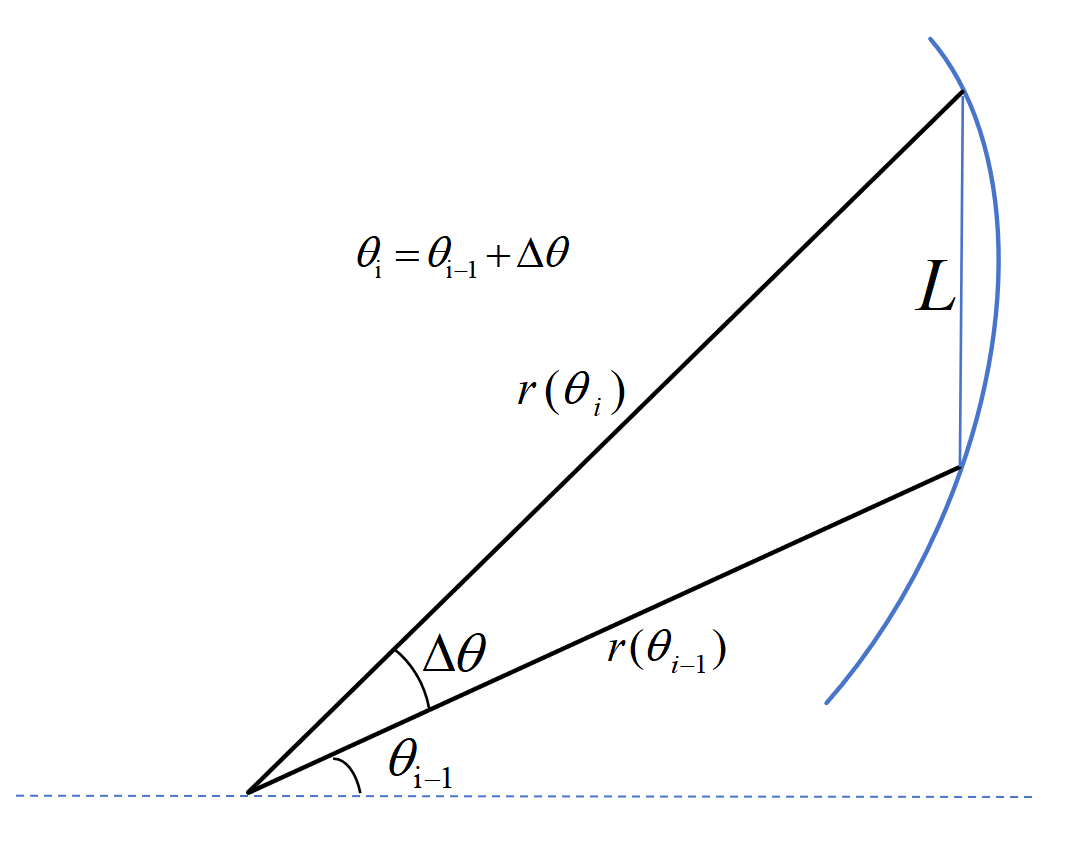
\includegraphics[width=0.5\linewidth]{cosine.png}
\end{figure}
\subsubsection{\textbf{问题1}后续龙身把手位置求解(近似圆弧法)}
下面介绍一种新解法,我们称之为近似圆弧法,其做法是在处理半径较大的螺线时我们可以将其等效为圆弧处理。理由是根据螺线轨迹方程,每当把手转过$2\pi$时,其半径衰减55cm,而当半径较大时(5—8m),
每次迭代一个有效板凳长作为螺旋线的弦所转过的角位移只有约0.35 rad/s。我们定义这种方法的误差度为$\delta_2$,根据计算,在时间不太大(300s内),后继把手数较多的情况下,
$\delta_2 \approx 10^{-4}$数量级左右,精度明显更好。
\par
下面给出一个具体算法:首先根据龙头极坐标解析表达式求得任意时刻$t$时的运动学状态,再应用近似圆弧法从任意时刻$t$的龙头坐标开始迭代,最终得到任意时刻“板凳龙”
各把手坐标数值,即任意时刻“板凳龙”的运动状态。仿真模拟算法步骤如以下\textbf{算法1}所述。
\par
\textbf{算法1:近似圆弧迭代法模拟舞龙的过程仿真:}
\newline
\noindent
\textbf{输出:}存储所有把手在所有整数时刻的位置,角位移矩阵。
\newline
\noindent
\textbf{S1:}创建两个矩阵,用行存储所有把手,用列存储所有要求解的时刻$t$。
\newline
\noindent
\textbf{S2:}根据先前求得的修正后龙头把手实时极坐标表达式(11),
可以得到任意时刻龙头把手的坐标,同时将求解结果填充进位置矩阵前两行。
\newline
\noindent
\textbf{S3:}下面从每个时刻$t$入手,即已经进入第一层关于时间$t$的循环后,从龙头把手进入循环迭代过程,
迭代对象和顺序依次是后续223个把手,从第2个把手开始循环迭代。对每个把手执行\textbf{S4}。
\newline
\noindent
\textbf{S4:}该步骤介绍从第i个把手到第i+1个把手的单次迭代循环过程。首先计算角位移的偏转值$\Delta \theta_i$,两个把手之间的螺旋线
近似作为圆弧处理,由圆周角三角形的几何公式,有:
\begin{equation}
    \Delta \theta_i=2\arcsin\frac{L}{2 r(\theta_i)}
\end{equation}
考虑到计算机编译器在求解反正弦数值的精确度和先前近似圆弧的误差,这里可以进一步作“以直代曲”的近似,直接将把手间有效连接长度
$L$作为这段圆弧长。由于先前将$r_(\theta_{i+1})$近似为$r_(\theta_{i})$会导致求解得到的$\Delta \theta_i$偏大,而这里以直代曲又使得$\Delta \theta_i$偏小,
且两者误差值位于同一数量级的水平,故作两次趋势相反的近似不仅简化了计算难度,也使得求出的$\Delta \theta_i$
精度更高。角位移偏转量方程为:
\begin{equation}
    \Delta \theta_i=\frac{L}{ r(\theta_i)}
\end{equation}
\par
再通过以下方程组:
\begin{align}
    \begin{cases}
        \theta_{i+1}=\theta_{i}+\Delta \theta\\
        r(\theta_{i+1})=11 \theta_{i+1}/40 \pi
    \end{cases}
\end{align}
\par
最终得到了第i+1把手的极坐标$(r(\theta_{i+1}),\theta_{i+1})$,可以通过一步平面直角坐标系投影得到最终的平面坐标$(r(\theta_{i+1}) \cos \theta_{i+1},r(\theta_{i+1}) \sin \theta_{i+1}) $。
\newline
\noindent
\textbf{S5:}对于时间循环$t$中的把手循环,循环执行\textbf{S4},由于龙头的存在,需要添加判断条件来区分不同板凳对应的有效连接长度。
\newline
\noindent
\textbf{S6:}因为已经求出了完整的各个时刻每个把手的位置信息,这使得我们有能力对全过程进行仿真模拟,只需要不断减小时间步长$t$,就可以逐渐趋近于一个连续过程。
可以借助计算机编译器,将全过程绘制成动画,这也为问题2判断相撞时间提供了依据。
通过计算机编译手段求得在给定时刻下把手的位置坐标,结果如表1所示。
\begin{table}[h!]
    \caption{位置结果}
    \centering
    \begin{tabular}{|c|c|c|c|c|c|c|}
    \hline
     & $0s$ & $60s$ & $120s$ & $180s$ & $240s$ & $300s$ \\
    \hline
    龙头 x (m) &8.8&5.796934&-4.090654&-2.953259&2.578971&4.431365 \\
    \hline
    龙头 y (m) & 0.000000 & -5.773329 & -6.300643 & 6.099638 &-5.363954&2.298233 \\
    \hline
     第1节龙身x& 8.366286&3.456016 & -6.111764 &-0.194664 & -191234  & 4.919684 \\
    \hline
     第1节龙身y& 2.819001 & -7.381867 &-4.310255  & 6.737217 & -5.906572&-0.466255  \\
    \hline
     第51节龙身x& -9.512018 & 5.486829 & -1.43511 & 3.932879 & 0.397575 & 0.227612 \\
    \hline
     第51节龙身y& 1.385148&4.680284& 6.28097   & 3.942671 & 4.512326 & -3.160608 \\
    \hline
     第101节龙身x& 2.841064 & 3.68234 & -5.07733 & -3.454000 & -2.47359 & 0.555436 \\
    \hline
     第101节龙身y& -9.938777& 4.902125 & 1.148161& 2.164192 & 0.20858 & 0.125698 \\
    \hline
     第151节龙身x& 10.877538& 0.124579 & -3.54136 & 0.133836 & -1.65013 & 2.255574 \\
    \hline
     第151节龙身y& 1.727014& -4.81315 & 0.409225 & -1.51431 & 0.002419& 10.325175 \\
    \hline
     第201节龙身x& 4.671434 & -2.35762 & 4.940488 & 0.532093 & -1.24801 & 8.958199 \\
    \hline
     第201节龙身y& 10.67392 & 1.802727 & 0.406542 & 0.73535 & 1.916431 & -4.124826 \\
    \hline
     龙尾(后)x& -5.427245 & 1.281067 & -0.406418 & 1.741699 & 0.019065 & -4.909683 \\
    \hline
     龙尾(后)y& -10.61406 & -0.94886 & -4.25146 & 0.734097 & 0.147523 & 8.173638 \\
    \hline
    \end{tabular}
    \label{tab:example}
\end{table}
\begin{figure}
    \caption{几个重要时刻“板凳龙”位置图}
    \centering    
    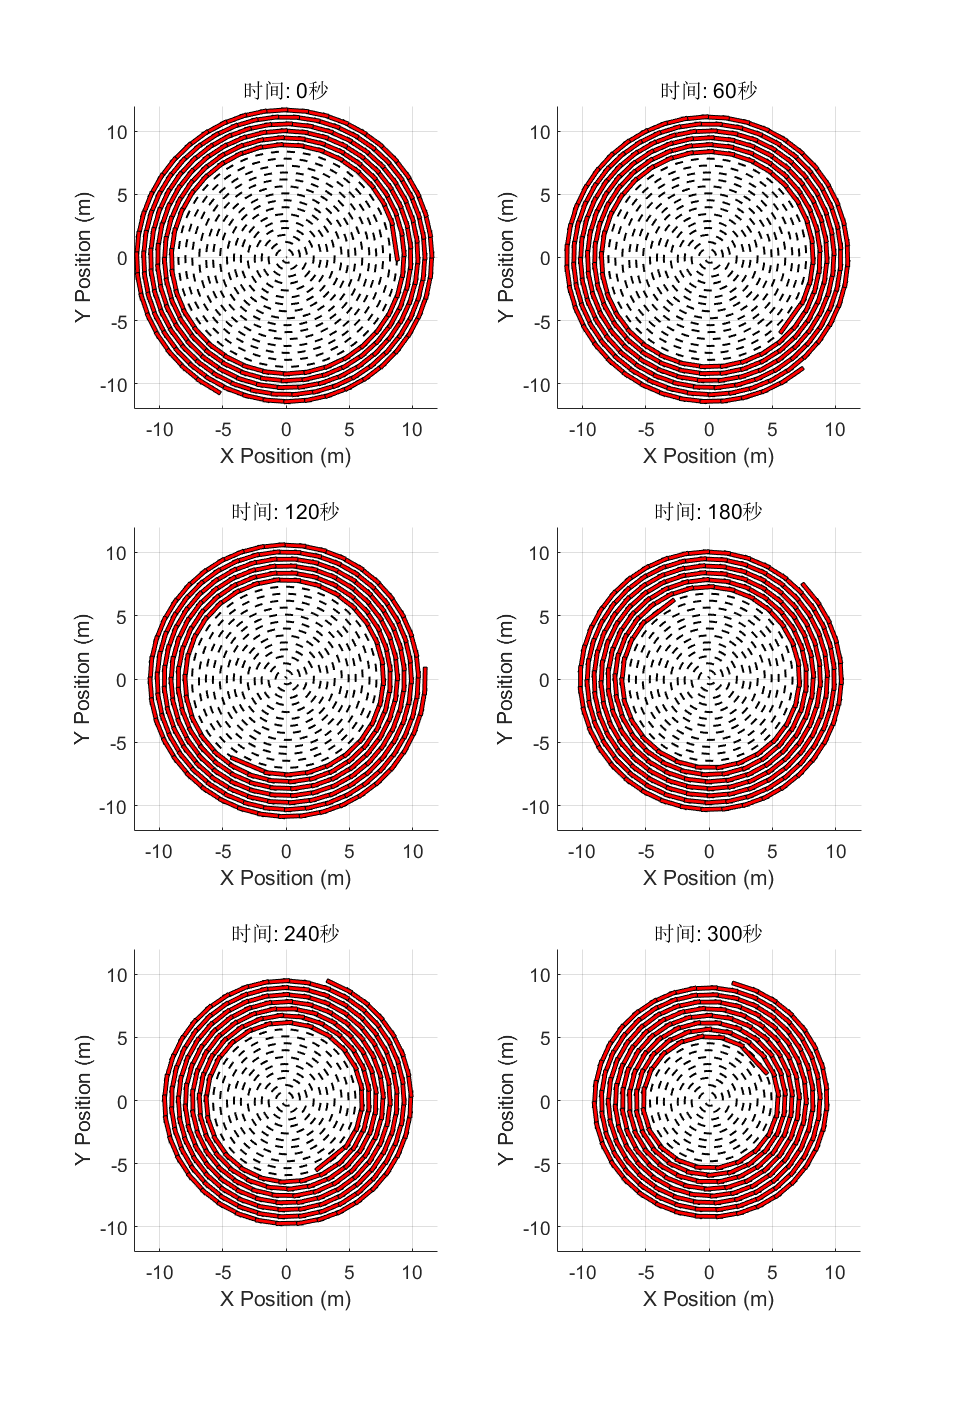
\includegraphics[width=0.83\linewidth]{drawing_t1_5_1_3.png}
\end{figure}

\subsubsection{\textbf{问题1}把手速度求解(差分法)}
由于在上一小节中已经可以对全过程进行模拟仿真,因此求解实时速度已经不再是问题。
根据速度定义公式,有:
\begin{equation}
    v_{ix}=\lim_{\Delta t \to 0}  \frac{\Delta x_i}{\Delta t} \quad v_{iy}=\lim_{\Delta t \to 0}  \frac{\Delta y_i}{\Delta t} 
\end{equation}
平方和求合速度:
\begin{equation}
    v_{i}=\sqrt{v_{ix}^2+v_{iy}^2}
\end{equation}
\par
由于无法对全过程进行连续的模拟仿真,我们只能取分立的值。重新设置一个关于时刻$t$新的
步长$ \delta t=0.0001$。用从这一时刻开始的微小时间内的平均速度近似代替在该时刻的瞬时速度。
因而有计算公式:
\begin{equation}
    v_{ix}(t)= \frac{ x_i(t+\delta t)-x_i(t)}{\delta t} \quad v_{iy}(t)= \frac{ y_i(t+\delta t)-y_i(t)}{\delta t} 
\end{equation}
\par
为了方便计算,把\textbf{算法1}封装进一个函数方便调用,接受的自变量为时间$t$,返回一个存储有该时刻所有点坐标的向量,通过这个函数不断向位置矩阵中写入向量。
在循环分别对$t$和$t+\delta$循环,得到两个存储有各个时刻和各个时刻后一段微小时间的矩阵,将两个矩阵相减并将全部元素除以$\delta t$,就得到了
所有把手的速度矩阵,题目要求时刻和把手的时刻数据如\表2,“板凳龙”位置图如图4。



\begin{table}[h!]
    \caption{速度结果}
    \centering
    \begin{tabular}{|c|c|c|c|c|c|c|}
    \hline
     & $0s$ & $60s$ & $120s$ & $180s$ & $240s$ & $300s$ \\
    \hline
    龙头 & 1.00005& 1.00006&1.00007&1.00008&1.00011&1.00015\\
    \hline
     第1节龙身& 1.00004 & 1.00004 & 1.00007 & 1.00005& 1.00006 & 1.00005 \\
    \hline
     第51节龙身& 0.99989 & 0.99984 & 1.00005 & 0.99966 &0.99945 & 0.99896 \\
    \hline
     第101节龙身& 0.99977 & 0.9997 & 0.99978 & 0.99942 & 0.99911 & 0.99845 \\
    \hline
     第151节龙身& 0.99969 &0.9996  &0.9996  & 0.99926 & 0.99889& 0.99816 \\
    \hline
     第201节龙身& 0.9996 & 0.99952 & 0.99947 & 0.99914 & 0.99875 & 0.99796 \\
    \hline
     龙尾(后)& 0.99949 & 0.99949 & 0.99934 & 0.9991 & 0.9987 & 0.9979\\
    \hline
    \end{tabular}
    \label{tab:example}
\end{table}

\subsection{\textbf{问题2}模型建立与求解}
\par 
为了判断在龙头到达极坐标原点前板凳之间是否会发生碰撞,以及找出碰撞的判据,同时求出具体碰撞的板凳节及其相应地坐标速度等运动状态,
需要建立一套有效的碰撞检测机制。由于“板凳龙”系统一共涉及到224节板凳,如果对每一节依次判断与其他223节是否相撞将极大地增加计算量,因此需要对这个预测碰撞系统做一些简化以降低计算复杂度。
比如先证明出某一节板凳的某个把手最容易和其他板凳发生碰撞。其次,由于在问题1中已经建立了“板凳龙”运动状态的实时仿真模拟模型,通过
对动画的观察,可以大致确定一个时间点$t_x$,
在$t_x$前一定不碰撞。
最后,我们需要考虑数据计算的误差。在具体计算过程中,随着循环迭代的次数不断增加,单次计算
产生的误差会随着循环次数增加不断累积,导致最终计算结果的偏差,因此需要找出一种方法尽可能地缩小误差。
\par
综上,我们建立一套“板凳间实时位置判断”的实时仿真模拟模型来解决这一问题。下面先介绍一种判断单个点与矩阵位置关系的方法——叉积法。

\subsubsection{建模准备:叉积法判断点与矩形位置关系}
由于在本问题中涉及对板凳碰撞的讨论,而板凳被等效成了一个长矩形,因此需要给出一个点是否位于另外一个矩形内部的判断依据。
如果在仿真模拟中发现在某一时刻$t_0$,存在某一个板凳的某个边界点出现在另一个矩形内部,则说明至少在$t_0$以前发生了碰撞。
\par
以下是叉积法的详细步骤:

\begin{figure}
    \caption{叉积法判断点是否在矩形内}
    \centering    
    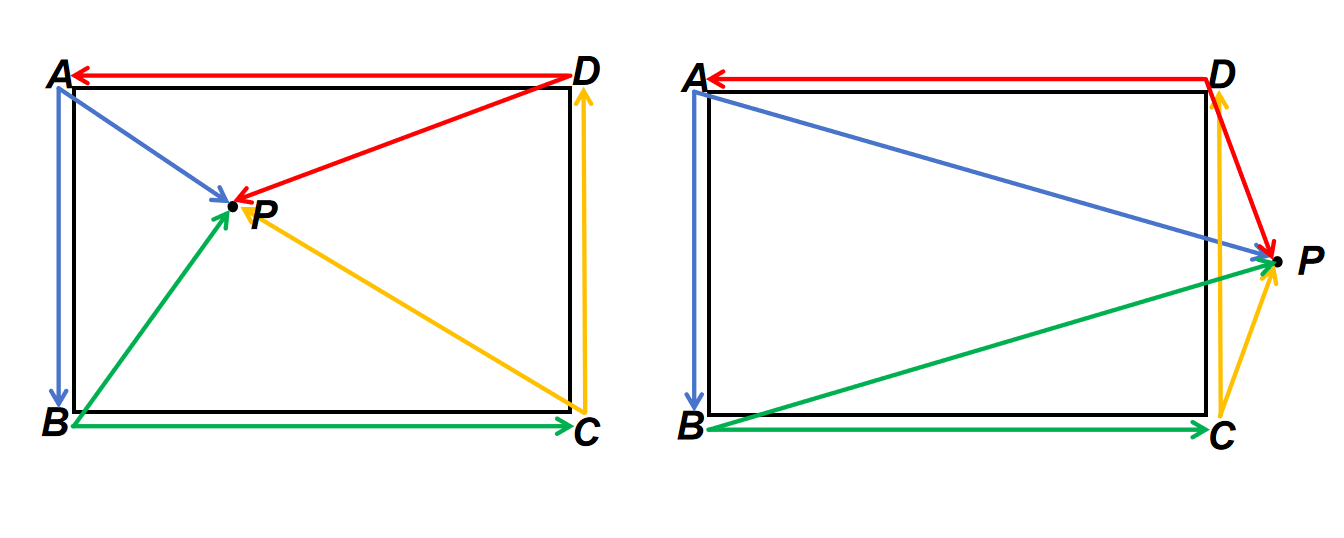
\includegraphics[width=0.95\linewidth]{chaji.png}
\end{figure}
\begin{enumerate}
    \item \textbf{确定矩形的顶点}:假设矩形的四个顶点为 $A$、$B$、$C$、$D$(按顺时针或逆时针顺序排列)。
    \item \textbf{计算点到矩形各边的叉积}:选择要判断的点 $P$。对于矩形的每一条边(假设边是由点 $A$ 到点 $B$),
    计算向量 $\overrightarrow{AB}$ 和向量 $\overrightarrow{AP}$ 的叉乘,其中 $\overrightarrow{AB}$ 是矩形边的向量,$\overrightarrow{AP}$ 是矩形顶点到点 $P$ 的向量。
    由于两个向量均位于平面上,所以仅需考虑叉乘在竖直方向上的正负,向量叉乘竖直方向竖直计算公式:

\begin{equation}
(\overrightarrow{AB} \times\overrightarrow{AP})_z=(x_B - x_A) \cdot (y_P - y_A) - (y_B - y_A) \cdot (x_P - x_A)
\end{equation}
    \item  \textbf{判断点关于矩形的位置}:如果点 $P$ 在矩形的每一边的相同一侧(即所有边的叉积结果都具有相同的符号),那么点 $P$ 就在矩形内部。
    因此,若平面内一点位于矩形内部,则满足以下方程组:

    \begin{equation}
        \begin{aligned}
            & \begin{cases}
                (\overrightarrow{AB} \times \overrightarrow{AP})_z > 0 \\
                (\overrightarrow{BC} \times \overrightarrow{BP})_z > 0 \\
                (\overrightarrow{CD} \times \overrightarrow{CP})_z > 0 \\
                (\overrightarrow{DA} \times \overrightarrow{DP})_z > 0
            \end{cases}
            \text{或} \quad
            \begin{cases}
                (\overrightarrow{AB} \times \overrightarrow{AP})_z < 0 \\
                (\overrightarrow{BC} \times \overrightarrow{BP})_z < 0 \\
                (\overrightarrow{CD} \times \overrightarrow{CP})_z < 0 \\
                (\overrightarrow{DA} \times \overrightarrow{DP})_z < 0
            \end{cases}
        \end{aligned}
    \end{equation}
\end{enumerate}    
\subsubsection{判断最先发生碰撞的板凳}
\par
我们可以进行以下三个断言:
\begin{enumerate}
    \item 一定是龙头那一节板凳最先与其他板凳发生碰撞。
    \item 以“板凳龙”前进方向为正方向,一定是龙头板凳所对应矩形的左前方边界点最先发生碰撞。
    \item 碰撞时刻,以龙头把手为起点,沿着螺线逆时针往回倒$ 5 \pi/2$,只需要检查角位移$\theta$
    与龙头把手角位移$\theta_1$ 相差不超过$ 5 \pi/2$的板凳把手,即与龙头相撞的板凳一定在这些板凳之间。
\end{enumerate}
\par
下面我们依次证明这三个断言使之成为正式的结论。
\begin{figure}
    \caption{300s后四个时刻图像}
    \centering    
    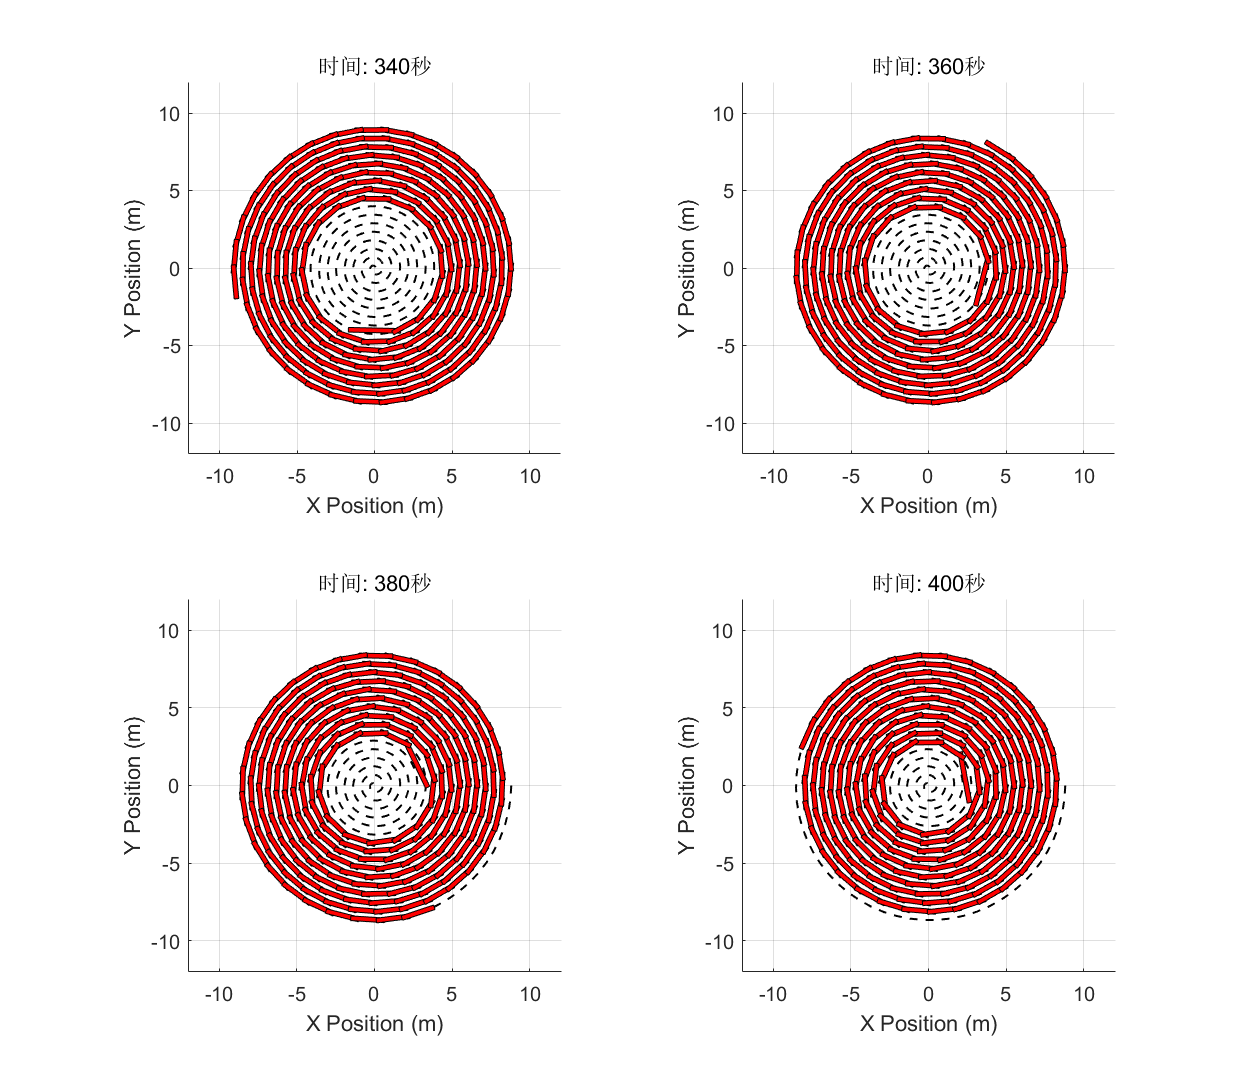
\includegraphics[width=1.0\linewidth]{5.2.2.png}
\end{figure}
\par
\textbf{结论1:证明:}使用反证法,假设存在龙头后续某块板凳(设其前把手标号为$i$)首先在时刻$t_2$与除龙头外的其他板凳相撞(设其前把手标号为$j$),如果是龙头,就是龙头除去边界点的四个边。
记录当前第i把手的角位移$\theta_i$。由于“板凳龙”的结构是由龙头牵引其他龙身运动,即龙头角位移$\theta_1$一定比$\theta_i$小,换言之
龙头一定在先前的某一时刻$t_1$到达过角位移为$\theta_i$的点,其中$t_1<t_2$。
由于龙头部分的长度$L_{head}$显然要长于龙身长度$L_{body}$,如果第i个龙身在$\theta_i$
处可以和其他板凳发生碰撞,那么龙头在$\theta_i$处也一定可以与后面的板凳发生碰撞。
这与所提假设矛盾。

\par
\textbf{结论2:证明:}
以“板凳龙”前进方向为正方向,我们依次标定矩形的四个边界点:依次分为左前、右前、左后、右后。首先先证明左后和右后边界点一定不可能是龙头首先与其他
板凳发生碰撞的把手。根据题目已知条件,螺距$p=55cm$,板凳后把手中心到后两个把手连线的距离(即与后板头的距离)为27.5cm。
可以作辅助线:相邻两条螺线的中间平分线。无论“板凳龙”盘入什么位置,后把手边界一定在相邻螺线的中心平分线内,更为通俗地说,这条螺线平分线完全可以将相邻螺线上的板凳矩形严格分割。
\par
下面接着证明,除了边界点以外的边不可能与其他板凳的任何点发生碰撞。依然使用反证法,假设
龙头矩形除了边界点以外的边可以与其他板凳的某个点发生碰撞。显然这个假设等价于结论1,矛盾所以舍去。
\par
最后证明,龙头右前把手不可能与其他板凳发生碰撞。根据实时仿真模拟图,龙头板凳右前边界点的相邻右侧螺线以及后续相邻的螺线上均不存在板凳节,故显然不可能发生碰撞。
\par
\textbf{结论3:证明:}一个显然的现象是,无论如何,碰撞只可能在相邻一个螺线范围内发生。即对于相碰的两个板凳,他们的角位移分别设为
$\theta_i$和$\theta_j$,由于他们不可能相隔一个螺线,故$\theta_i$和$\theta_j$的差值
$\Delta \theta_{ij}=\theta_i-\theta_j$一定在$2 \pi$左右,为了保险起见,我们将这一数值设置为$5/2 \pi$。
根据实时仿真模拟可以判断出,“板凳龙”系统在第400s时不会发生碰撞,此时综合考虑龙头把手对应的弧度及其螺旋半径长作放大估算,我们只需要从第1节龙身板凳遍历到第18龙身板凳即可。
\par
在正式建立检测模型前,为了尽可能减少我们的计算复杂度,提高计算效率,首先得出了以上三个结论。
根据第一个结论,我们可以减少一轮循环,不需要再去检查224个板凳的四个边界点中的每一个点是否与其他223个板凳相碰。根据第二个结论,我们
不再需要一一遍历龙头板凳四个边界点,而是只需要去判断左前边界点是否与后续的板凳发生碰撞。而最后一个结论大大减少了检查循环中所需要的轮数,
每轮遍历只需要对龙头板凳后十八节板凳进行判断即可。

\subsubsection{碰撞条件和板凳矩形区域求解}
\par
根据上一小节的三个定理,我们把板凳间的相互碰撞问题转化成了点与矩形的碰撞问题,也就是点与矩阵的位置关系问题,可以通过叉积法解决。
设有点$ (x_0,y_0)$和矩形$ABCD$,矩形的四个边界点坐标依次为
$(x_{11}, y_{11}),(x_{12}, y_{12}),(x_{21}, y_{21}),(x_{22}, y_{22})$。
我们记区域$H$为由这四个点连线所形成的矩形,则关于碰撞条件,有下面的关系式(以相碰为例):
\begin{equation}
    H= \begin{bmatrix}
        (x_{11}, y_{11}) & (x_{12}, y_{12}) \\
        (x_{21}, y_{21}) & (x_{22}, y_{22})
        \end{bmatrix}
        \quad (x_0,y_0) \in H
\end{equation}
\par
将上面的式子用叉积法转换成坐标表达式,(两个方程组只满足其中一个):
\begin{equation}
    \begin{aligned}
        &\begin{cases}
            (x_{11} - x_{12}) \cdot (y_{0} - y_{11}) - (y_{11} - y_{12}) \cdot (x_{0} - x_{11}) > 0 \\
            (x_{12} - x_{21}) \cdot (y_{0} - y_{12}) - (y_{12} - y_{21}) \cdot (x_{0} - x_{12}) > 0 \\
            (x_{21} - x_{22}) \cdot (y_{0} - y_{21}) - (y_{21} - y_{22}) \cdot (x_{0} - x_{21}) > 0 \\
            (x_{22} - x_{11}) \cdot (y_{0} - y_{22}) - (y_{22} - y_{11}) \cdot (x_{0} - x_{22}) > 0 \\
        \end{cases} 
    \end{aligned}
\end{equation}
    
\begin{equation}
    \begin{aligned}
        \begin{cases}
            (x_{11} - x_{12}) \cdot (y_{0} - y_{11}) - (y_{11} - y_{12}) \cdot (x_{0} - x_{11}) < 0 \\
            (x_{12} - x_{21}) \cdot (y_{0} - y_{12}) - (y_{12} - y_{21}) \cdot (x_{0} - x_{12}) < 0 \\
            (x_{21} - x_{22}) \cdot (y_{0} - y_{21}) - (y_{21} - y_{22}) \cdot (x_{0} - x_{21}) < 0 \\
            (x_{22} - x_{11}) \cdot (y_{0} - y_{22}) - (y_{22} - y_{11}) \cdot (x_{0} - x_{22}) < 0 \\
        \end{cases}
    \end{aligned}
\end{equation}
\par
在具体代码实现时,可以将以上判断过程封装进一个函数,接口为龙头板凳左前边界点坐标和后续板凳矩形边界点坐标。
下面的问题在于,如何求出所需要的相应矩形边界点坐标,即求出第$i$个把手所处板凳四个边界点坐标矩阵
$ \begin{bmatrix}
    (x_{ifl}, y_{ifl}) & (x_{ifr}, y_{ifr}) \\
    (x_{ibl}, y_{ibl}) & (x_{ibr}, y_{ibr})
\end{bmatrix} $。
由于相邻把手分别是一条板凳的前后把手,因此只要知道一对相邻板凳把手的坐标,就可以将该板凳的四个边界点坐标完全解出。
\par
由于已经求出各时刻所有把手的位置坐标,因此在求解边点时不再需要通过循环迭代,只需要传入求好的位置矩阵即可。
根据图6,对于第i节板凳(前把手为第i个把手),需要求出能够表示其走向的方向向量,定义$\vec{e_i}$来表示第i块板凳的方向(从第i个把手指向第i+1个把手),$\vec{f_i}$表示其法向有:
\begin{equation}
     \vec{e_i}=\frac{(x_{i+1}-x_i,y_{i+1}-y_i)}{\sqrt{(x_{i+1}-x_i)^2+(y_{i+1}-y_i)^2}}
\end{equation}
\begin{equation}
    \vec{f_i}=\frac{(y_{i}-x_{i+1},x_{i+1}-x_i)}{\sqrt{(x_{i+1}-x_i)^2+(y_{i+1}-y_i)^2}}
\end{equation}
\par
下面可以通过$\vec{e_i}$结合其他相应的参数如板宽$w$,板头板尾长$d $可以求出该矩形四个边界点坐标:
\begin{equation}
    (x_{ifl}, y_{ifl})=(x_i,y_i)-d \cdot \vec{e_i} -\frac{w}{2} \cdot\vec{f_i}
\end{equation}
\begin{equation}
    (x_{ifr}, y_{ifr})=(x_i,y_i)-d \cdot \vec{e_i} +\frac{w}{2} \cdot\vec{f_i}
\end{equation}
\begin{equation}
    (x_{ibl}, y_{ibl})=(x_{i+1},y_{i+1})+d \cdot \vec{e_i} -\frac{w}{2} \cdot\vec{f_i}
\end{equation}
\begin{equation}
    (x_{ibr}, y_{ibr})=(x_{i+1},y_{i+1})+d \cdot \vec{e_i} +\frac{w}{2} \cdot\vec{f_i}
\end{equation}

可以将上述求解过程直接封装进一个函数,在函数中定义一个矩阵直接存储所有把手在所有时刻下对应板凳边点的坐标。
\begin{figure}
    \caption{矩形边点求解示意图}
    \centering    
    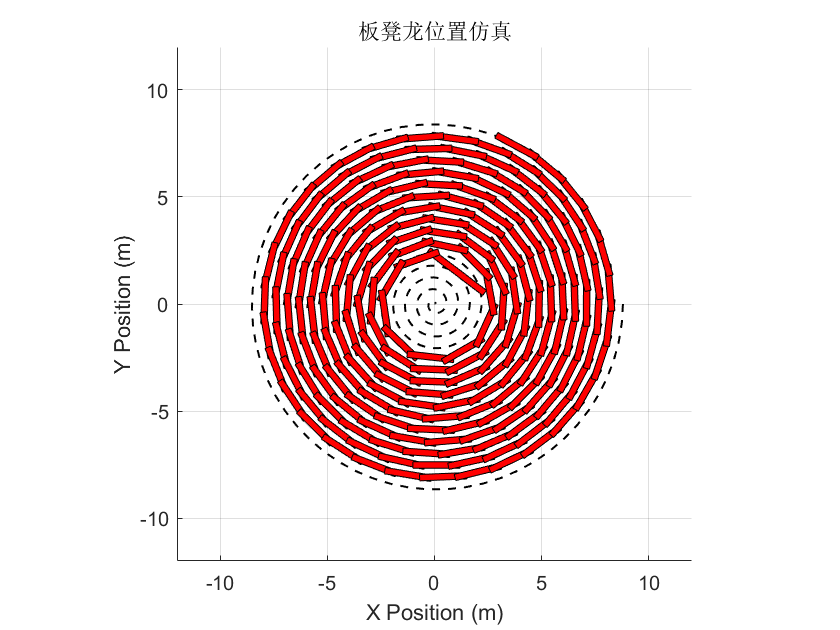
\includegraphics[width=0.9\linewidth]{5.2.4.png}
\end{figure}
\begin{figure}
    \caption{矩形边点求解示意局部图}
    \centering    
    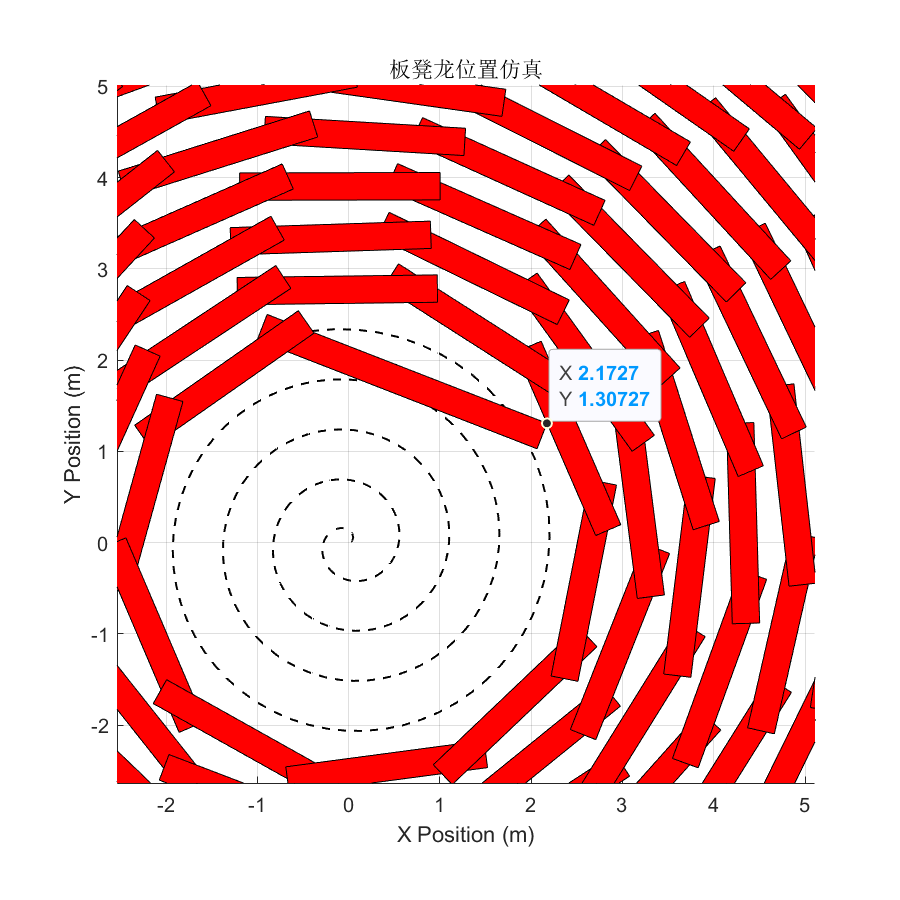
\includegraphics[width=0.65\linewidth]{drawing_5.4.2.8.png}
\end{figure}
\subsubsection{判断板凳间实时位置的仿真模拟模型和结果}
经过以上几个小节的铺垫,判断板凳间实时位置的仿真模拟模型已经呼之欲出了。我们可以只通过两轮循环就求解出
所有的龙头板凳左前边点在任意时刻关于是否与后续板凳发生碰撞的布尔值矩阵。我们通过一个算法来描述这个
“判断板凳间实时位置的仿真模拟模型”。为了后续得到精确的碰撞时刻,同时提高仿真模拟的精确程度,我们设置时间步长为$\Delta t=0.01$。
\par
\textbf{算法2:判断板凳间实时位置的仿真模拟模型:}
\newline
\noindent
\textbf{输入:}存储所有把手在所有时刻的位置矩阵,板凳边点矩阵。
\newline
\noindent
\textbf{输出:}“板凳龙”实时运动状态动画,碰撞时刻,碰撞时刻下各个把手的位置与速度矩阵。
\newline
\noindent
\textbf{S1:}进入第一轮循环,每一个循环节对应一个时刻。时刻$t$从400s开始,以$\Delta t$的步长逐渐增加,然后再进入一轮循环。
\newline
\noindent
\textbf{S2:}进入第二轮循环,每一个循环节对应一个板凳的判断过程,只需要遍历从龙头板凳开始的18节龙身板凳,由此进入第三轮小遍历。
\newline
\noindent
\textbf{S3:}进入第三轮小遍历,依次遍历一个板凳矩形的四个把手,对于每个板凳边点,调用叉积法判断点与矩形相碰与否,同时传入龙头板凳左前点坐标。
\par
根据上述算法不难编程求解得到答案,最终求得在时刻$t_{crash}=413.36s$与第8节龙身,即从龙头开始的第九节板凳龙发生碰撞,此时龙头前把手的坐标为(2.1727, 1.30727)。
相应地碰撞时刻全局状态图和局部状态图分别如图7,图8所示。此时龙头前把手、龙头
后面第 1、51、101、151、201 条龙身前把手和龙尾后把手的位置和速度如表3所示。
\begin{table}[h!]
    \caption{碰撞时刻对应}
    \centering
    \begin{tabular}{|c|c|c|c|}
    \hline
     & $x(m)$ & $y(m)$ & $v(m/s)$  \\
    \hline
    龙头 & 1.856699& 1.275657&1.000755\\
    \hline
     第1节龙身& -0.700321 & 2.257706 & 0.998250 \\
    \hline
     第51节龙身& 2.489526 & 3.731819& 0.988250  \\
    \hline
     第101节龙身& -1.960849 & -5.546337 & 0.986675  \\
    \hline
     第151节龙身& -0.569067&-6.982230  &0.986033\\
    \hline
     第201节龙身& -7.962845 & 0.361181 & 0.985683  \\
    \hline
     龙尾(后)& 2.530747 & 7.968352 & 0.985576\\
    \hline
    \end{tabular}
    \label{tab:example}
\end{table}


\subsection{\textbf{问题3}模型建立与求解}
问题三要求我们确定最小螺距,使得龙头前把手能够沿着相应的螺线盘入到调头空间的边界。这个问题本质上是在寻找一个平衡点,即螺距既要足够小以满足题目所需要求,又要足够大以避免在龙头前把手到达调头空间前发生板凳之间的碰撞。我们需要考虑的关键因素包括螺线的几何特性、舞龙队的物理结构以及调头空间的限制。\par
\subsubsection{\textbf{问题3}模型建立}
在问题二我们已经求出了当螺距p=0.55m时第一次发生碰撞时的时间,以及各把手在第一次碰撞时的位置和速度信息,若将p设为参数,则我们可以通过传入参数p,求得在任意螺距下第一次发生碰撞时各把手的位置和速度参数。现在我们须求最小的螺距,使得龙头前把手在发生碰撞之前就已经到达了调头空间的边界。若此时假设没有调头空间,龙头依然按盘入螺旋线盘入,可知,当之后的某一时刻发生碰撞时,龙头的前把手一定位于调头空间之内。若此时龙头前把手的坐标为($x_1$, $y_1$),则一定满足:
\begin{equation}
    x_1^2 + y_1^2 \leq R^2
\end{equation}
\begin{figure}
    \caption{碰撞时龙头与中心距离示意图}
    \centering    
    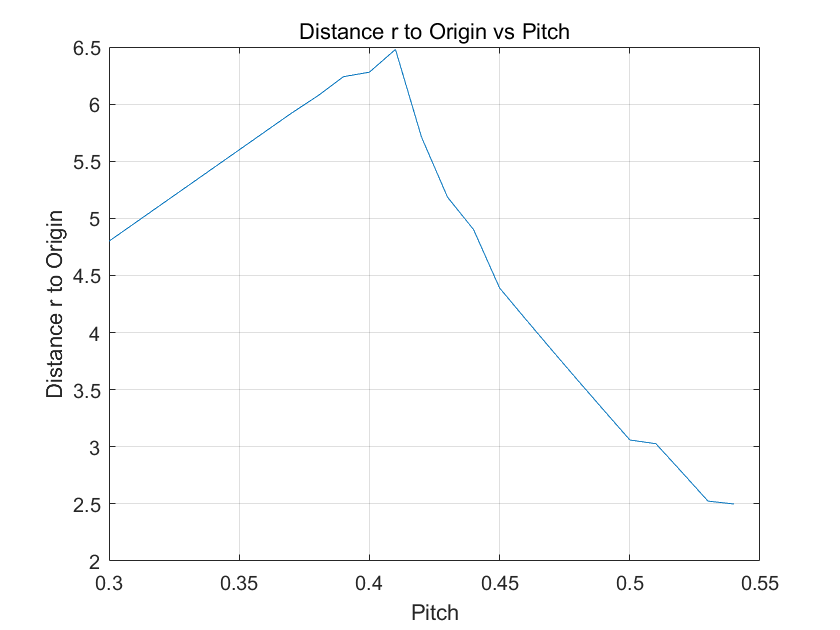
\includegraphics[width=0.7\linewidth]{5.3.4.png}
\end{figure}
其中,R为调头空间的半径。显然,由于螺距越小发生碰撞的可能性越大。因此,我们可以从螺距p=0.55开始,以一个较为粗略的步长不断减小螺距,求出当前螺距下第一次发生碰撞时龙头前把手到圆心的距离。结果如图9所示,随着螺距逐渐增大,龙头与某一部分龙身发生碰撞时距离中心的距离也有所不同。可以看出,随着螺距逐渐增大,碰撞时龙头距离中心的距离先增加再减小。不难发现,螺距从0.3m到0.41m左右时,龙头出发点与中心的距离不断增大;当螺距再增加时,由于间距过大,龙头与龙身之间更加难以碰撞,因此要到靠近中心的位置才可能发生碰撞。
\par
我们的目标是求得最小的满足式(34)的螺距$p_{min}$。由于R=4.5m,从图9可以组略估计:$p_{min}$位于0.4到0.45这一区间内。因此我们可以从p=0.4m开始,不断增大进行较高精度的搜索,直至根据当前p求出的($x_1$,$y_1$)满足式(34)方程。
\par

\subsubsection{\textbf{问题3}模型的求解}
为了实现上述螺距优化模型,我们设计了一个迭代优化算法。这个算法的主要步骤如下:
首先,我们初始化系统参数,包括螺距的搜索范围、龙头和龙身的长度、把手间距等。然后,我们遍历所有的螺距来搜索满足条件的螺距。在每次迭代中,我们都会模拟舞龙队的盘入过程,检查第一次发生碰撞时龙头前把手是否位于调头空间之内,并根据结果调整螺距的搜索范围。这个过程会一直持续,直到找到满足条件的最小螺距或达到预设的迭代次数上限。具体来说,算法的步骤可以分为以下几步。
\par
\begin{figure}
    \caption{不同时刻矩形边点示意图}
    \centering    
    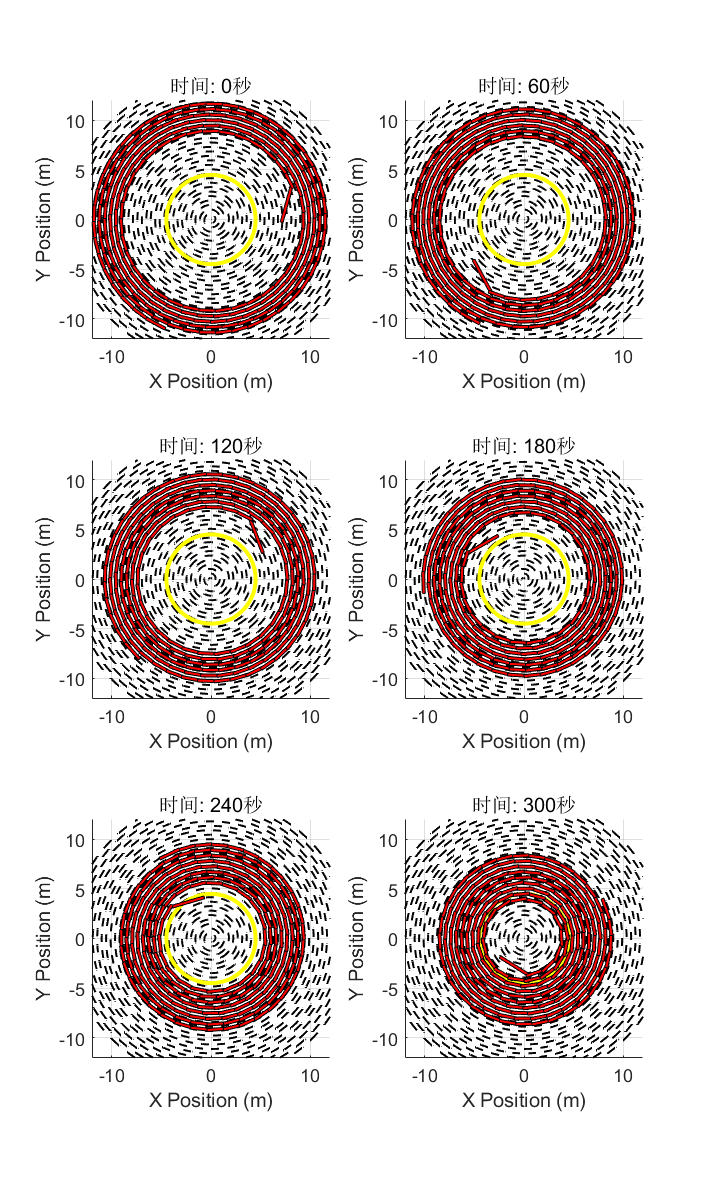
\includegraphics[width=0.7\linewidth]{5.3.2.png}
\end{figure}
\par
\textbf{算法3:迭代优化调整螺距:}
\newline
\noindent
\textbf{S1:}初始化参数:初始化碰撞时间,给出螺距初始值为0.40,设定螺距增加的步长为0.01m,给出调头空间的半径R=4.5m,定义最大螺距为1.0m,防止无限循环。开始主循环。
\newline
\noindent
\textbf{S2:}在每一个循环节中,我们会进入一个子循环体,从时刻0开始不断前进,调用之前问题求得的函数来计算每时刻所有把手的位置,调用算法3中封装函数体“叉积法”检测当前位置是否发生了碰撞。若检测成功,则跳出子循环体。
\newline
\noindent
\textbf{S3:}判断当前龙头前把手位置是否位于调头空间内。若判断成功,则输出当前的螺距,结束算法。反之,将当前螺距增加一个步长,回到步骤\textbf{S2}。
\par
通过调用算法3,我们求出$p_{min}$=0.45m,即当p < 0.45m时,龙头前把手在还未进入调头空间时就已经由于碰撞而停止前进了。

\par

\begin{figure}
    \caption{碰撞时矩形边点示意图}
    \centering    
    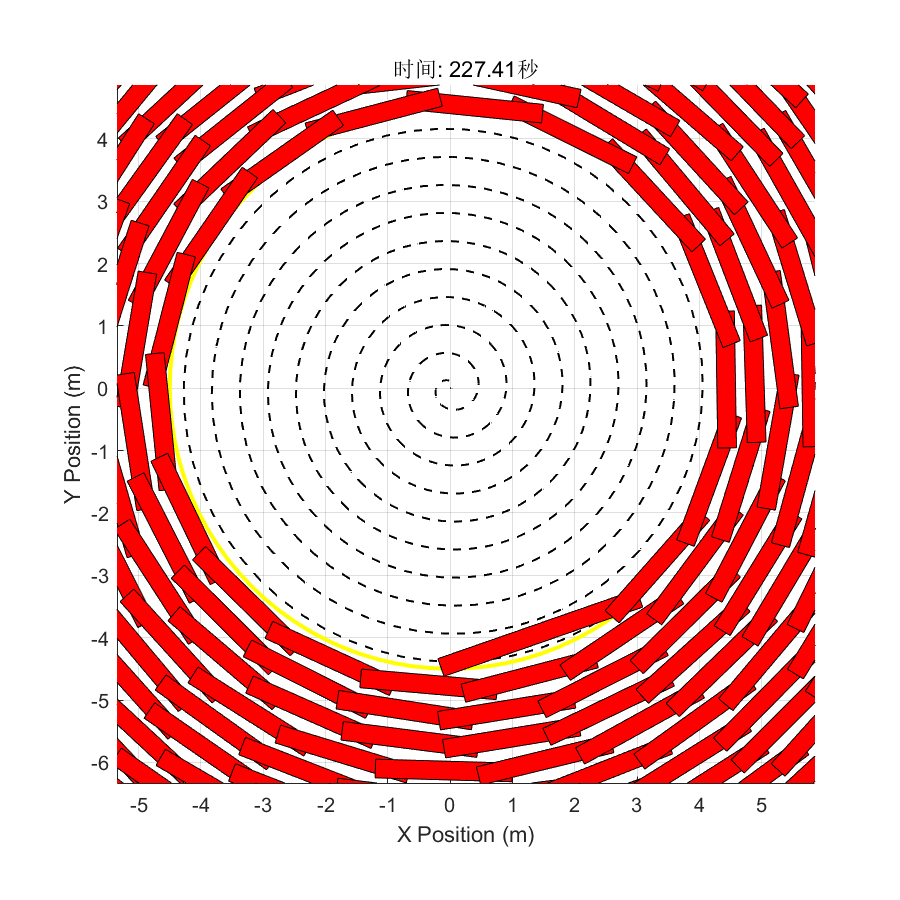
\includegraphics[width=0.8\linewidth]{5.3.3.png}
\end{figure}
\par
\subsubsection{\textbf{问题3}仿真分析和验证}
将当前螺距设置为0.45m,我们从0时刻开始模拟各板凳龙的运动。中间过程如图10所示,可以看出,当螺距减少时,龙头的有效长度$L_{eff1}$和龙身有效长度$L_{eff2}$的差异被放大。具体表现在龙头前把手同龙头后把手之间的角位移增加,两个把手之间相隔了多圈螺旋线,而后面的龙身把手则依旧紧密。同时,从图中可以看出,碰撞发生在180s到240s之间。通过缩小迭代的步长,我们可以求出第一次碰撞具体发生在227.41s:龙头左前把手同第十六节龙身发生碰撞。
\par
在227.41s碰撞时刻的局部示意图如图11所示,从中可以验证,此时龙头左前角同第十六节龙身的有边界发生碰撞。从仿真可以看出,我们的结果是准确的,且具有较高的精度。

\par


\subsection{\textbf{问题4}模型建立与求解}
\par
对于给定的掉头半径与两端掉头圆弧的半径比值,可以列出非线性方程,通过赋予计算机若干初始解的方法不断优化进而得到全局最优解。
为了尽可能减小“板凳龙”在掉头圆内的掉头路程,可以放开两端掉头圆弧半径比值为2的严格限制,这样使得原本只存在最优解(数值解)的
方程问题释放了一个自由度成为了一个动态规划问题,通过结合计算机数值求解与动态路径规划与优化,可以得到使得掉头路程尽可能短的两端掉头圆弧的数值解。
该问题的关键在于如何设计一个更优的掉头曲线,在保证掉头过程更加高效的情况下同时保证运动的连续性和解的精确性。
\subsubsection{严格限制半径比值1:2的掉头圆弧方程求解}
示例情形如图
~\ref{fig:spiral_and_arc} 
所示。
题目中已经给定了螺距大小为$p=1.7m$,相应地,盘入螺线轨迹为:
\begin{equation}
    r(\theta)=\frac{1.7 \theta}{2 \pi}
\end{equation}
又因为掉头区域半径为$R=4.5m$,故代入求解得到“板凳龙”盘入到掉头区域时的位置$P_1(x_1,y_1)$极坐标为$(4.5,16.630)$,即角位移$\theta_0=16.630$,通过平面直角坐标系投影得到$P_1$平面直角坐标为$(-2.7119,-3.5911)$。
根据盘出螺线与盘入螺线的中心对称性质,得到“板凳龙”盘出螺线和掉头区域的交点$P_2(x_2,y_2)$相应坐标依次$(2.7119,3.5911)$。
\begin{figure}
    \caption{盘入盘出螺线与掉头圆弧示意图}
    \centering    
    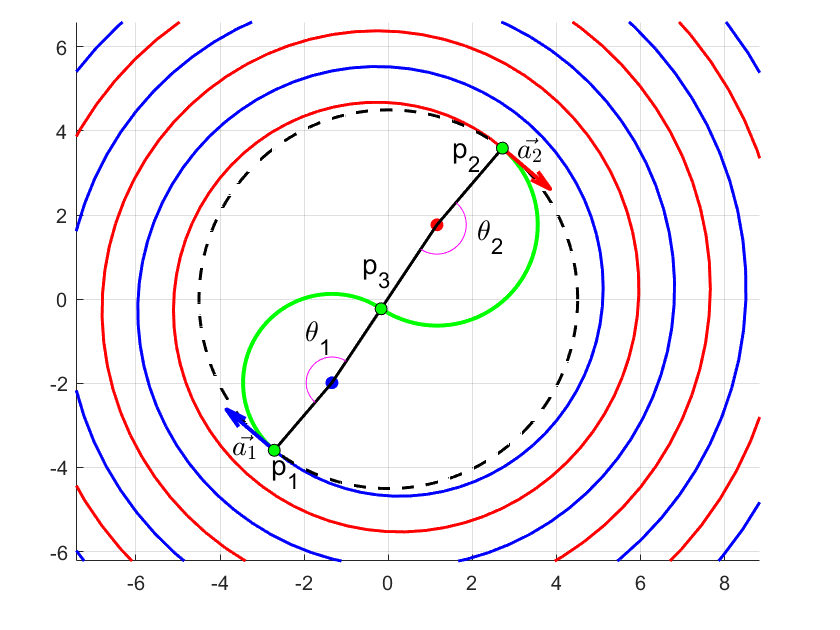
\includegraphics[width=0.7\linewidth]{drawing_5.4.1.1.png}
    \label{fig:spiral_and_arc} % 添加图像标签
\end{figure}
\par
下面设出各种未知数,并根据题目所给条件列出约束方程:掉头圆弧所对应的圆心坐标$O_1,O_2$,
半径分别为$ (x_{o1},y_{o1})$ ,$ (x_{o2},y_{o2})$和$r_1,r_2$,设两端圆弧线交点为$P_3$。
由于两端圆弧在内部相切,故它们的圆心连线长度应恰好等于半径之和:
\begin{equation}
    d(O_1,O_2)=\sqrt{(x_{o1}-x_{o2})^2+(y_{o1}-y_{o2})^2}=r_1+r_2
    \label{eq:distance1}
\end{equation}
\par
两端圆弧在掉头区域的边界同盘入盘出螺线相切,故下面推导边界处的相切方程表达式。
记$\vec{a_1}$为把手盘入螺线在角位移$\theta_1$处的切线方向向量,有:
\begin{equation}
    \vec{a_1}=-(\frac{dx}{d \theta},\frac{dy}{d \theta})=-(\frac{d \frac{1.7}{2 \pi} \theta \cos \theta}{d \theta},\frac{d \frac{1.7}{2 \pi} \theta \sin \theta}{d \theta})
=-\frac{1.7}{ 2 \pi}(\cos \theta_0-\theta_0 \sin \theta_0,\sin \theta_0+\theta_0 \cos \theta_0)
\end{equation}
\par
这里由于把手顺时针向原点盘入,故描述把手在该点方向向量时需要添加负号。
根据圆的相关知识,圆$O_1: (x-x_{O1})^2+(y-y+{O1})=r_1^2$在$\theta_0,P_1(x_1,y_1)$的切线方向向量为
$\vec{b_1}=(y_1-y_{O1},x_{O1}-x_1)$。由于在该点两条曲线相切,因此它们的方向向量平行,即$\vec{a_1} \parallel \vec{b_1}$,相应坐标表达式为:
\begin{equation}
    \frac{x_{O1}-x_1}{y_1-y_{O1}}=\frac{\sin \theta_0+\theta_0 \cos \theta_0}{\cos \theta_0-\theta_0 \sin \theta_0}
    \label{eq:qiexian1}
\end{equation}
同样的,对于盘出螺线我们也有平行的结论:
\begin{equation}
    \vec{a_2}=-\vec{a_1}=\frac{1.7}{ 2 \pi}(-\cos \theta_0+\theta_0 \sin \theta_0,-\sin \theta_0-\theta_0 \cos \theta_0)
\end{equation}
\begin{equation}
   \vec{b_2}=(-y2-y_{O2},x_1+x_{O2}) \parallel \vec{a_2}
\end{equation}

\begin{equation}
    -\frac{x_{O2}+x_1}{y_2+y_{O2}}=\frac{-\sin \theta_0-\theta_0 \cos \theta_0}{-\cos \theta_0+\theta_0 \sin \theta_0}
    \label{eq:qiexian2}
\end{equation}
\par
又因为$P_1,P_2$本身分别位于$O_1,O_2$上,有:
\begin{equation}
    (x_{1}-x_{o1})^2+(y_{1}-y_{O1})^2=r_1^2
    \label{eq:oncircle1}
\end{equation}
\begin{equation}
    (x_{2}-x_{o2})^2+(y_{2}-y_{O2})^2=r_2^2
    \label{eq:oncircle2}
\end{equation}
\par
再加上题目给出的有关半径的严格限制:
\begin{equation}
    r_1=2r_2
    \label{eq:radius}
\end{equation}
\par
到现在为止,我们已经根据几何关系得出了所有的约束方程,现在结合方程与未知数个数来判断
方程的类别。
\par
我们选取式 \eqref{eq:distance1} 
\eqref{eq:qiexian1}
\eqref{eq:qiexian2}
\eqref{eq:oncircle1}
\eqref{eq:oncircle2}
\eqref{eq:radius}
组成方程组,这里的未知数由$x_{O1},y_{O1},
x_{O2},y_{O2},r1,r2$共计6个组成,因此我们可以判断,
理论上该方程由最优的唯一解。由于方程组的类型为非线性方程组,可行的求解方法只有
只有设定若干有效初始解,通过计算机求解器从这些初始解出发,不断向周围优化迭代循环,直至找到一个最优化的数值解。
\par
经过计算机求解器求解,得到了两组较为精确的数值解,这两组呈现中心对称关系,解为:
\begin{align}
    \begin{cases}
        \text{圆}O_1 \quad (-0.7600,-1.3058) \quad r_1=3.0054 \quad \theta_1=3.0215\\
        \text{圆}O_2 \quad (1.7358,2.4485) \quad r_2=1.5027 \quad \theta_2=3.0215\\
    \end{cases}
\end{align}
\begin{align}
    \begin{cases}
        \text{圆}O_1 \quad (1.7358,2.4485) \quad r_1=1.5027 \quad \theta_1=3.0215\\
        \text{圆}O_2 \quad (-0.7600,-1.3058) \quad r_2=3.0054 \quad \theta_2=3.0215\\
    \end{cases}
\end{align}
\par
可视化结果如图
~\ref{1:2} 
所示。
\begin{figure}
    \caption{半径比1:2的情形}
    \centering    
    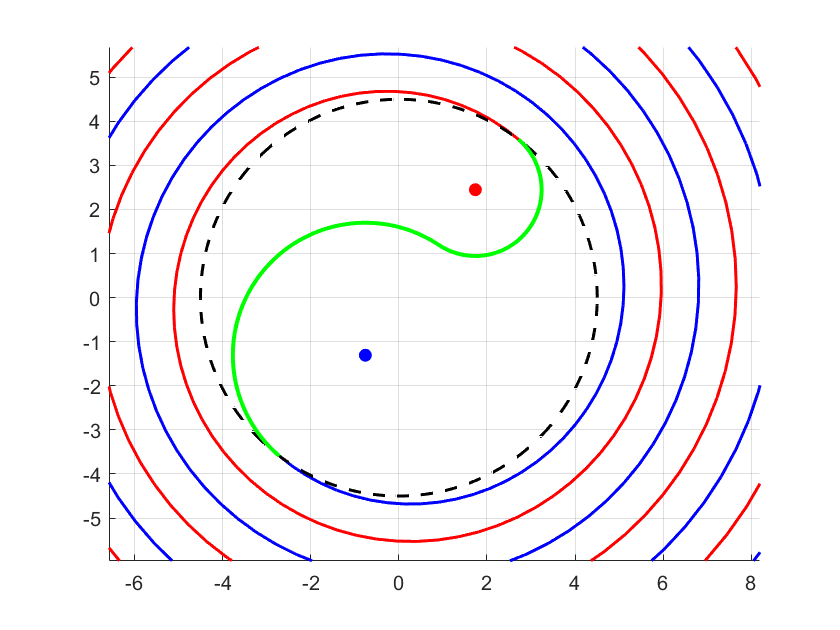
\includegraphics[width=0.7\linewidth]{drawing_5.4.1.2.png}
    \label{1:2}
\end{figure}
\par
这里还有个有趣的现象,那就是半径比在某个范围内变化时,大部分有$\theta_1=\theta_2$,例如,当半径比$\alpha \in [1.5,3]$时($\alpha=r_2  /r_1$或$r_1/r_2$),经过离散检验,
$\theta_1=\theta_2=3.0215$成立的可能性很高。
\subsubsection{放开半径比值限制优化最短路径}
如果要进一步优化圆弧,使得掉头的路程长度最小,唯一的选择是放开对半径比值严格为1:2的限制,
即我们的方程组除去了式\eqref{eq:radius},剩下 式\eqref{eq:distance1} 
\eqref{eq:qiexian1}
\eqref{eq:qiexian2}
\eqref{eq:oncircle1}
\eqref{eq:oncircle2}。
少去的方程释放了一个自由度,使得该问题变成了在给定约束条件下的一个非线性规划问题。
如图
~\ref{fig:spiral_and_arc} 
所示,掉头曲线长度表达式与规划目标为:
\begin{equation}
    \text{min} \quad S=\theta_1 r_1+\theta_2 r_2
\end{equation}
\par
通过对未知元和约束方程个数分析我们知道,这个非线性动态规划问题中
一共涉及4个未知元,而与这些未知元相关的方程个数只有3个,因此只有一个自由度,但方程解的个数变成了无穷。
\par
仍然延续上一小节中的各个字母变量符号。
由于两个螺旋线相切于$P_3$,可以给出$P_3$的两种不同表达式,最终令其相等。
由题意可知,圆$O_1$在$P_1$的切线向量为$\vec{a_1}$,
现在将方向向量$\vec{a_1}$顺时针方向旋转$90^\circ$,根据坐标顺时针旋转$\phi$角公式:
\begin{equation}
    \begin{bmatrix}
        x' \\
        y'
        \end{bmatrix}
        =
        \begin{bmatrix}
        \cos\phi & \sin\phi \\
        -\sin\phi & \cos\phi
        \end{bmatrix}
        \begin{bmatrix}
        x \\
        y
        \end{bmatrix}
\end{equation}
\par
旋转后的向量$\vec{a_1}$是$\overrightarrow{a_{irot}}$:
\begin{equation}
\overrightarrow{a_{irot}}=
        \begin{bmatrix}
        0 & 1 \\
        -1 & 0
        \end{bmatrix}
        \vec{a_1}
\end{equation}
\par
容易知道$\overrightarrow{P_1 O_1}$同$\overrightarrow{a_{irot}}$
方向相同。又因为圆$O_1$半径是$r_1$,因此有:
\begin{equation}
    \overrightarrow{P_1 O_1}=r_1 \cdot \frac{\overrightarrow{a_{irot}}}{|\overrightarrow{a_{irot}}|}
\end{equation}
\par
通过这个方程可以求出对应的点坐标,我们通俗地表示为:
\begin{equation}
    O_1=P_1+\overrightarrow{P_1 O_1}
\end{equation}

由于$\overrightarrow{O_1 P_3}$ 为$\overrightarrow{O_1 P_1}$
顺时针旋转$\theta_1$得到,因此有:
\begin{equation}
    \overrightarrow{O_1 P_3}=
    \begin{bmatrix}
        \cos\theta_1 & \sin\theta_1 \\
        -\sin\theta_1 & \cos\theta_1
        \end{bmatrix}
            (-\overrightarrow{ P_1 O_1})
    \end{equation}
\par
该式子可以得到$P_3$的坐标表达式:
\begin{equation}
    P_3=O_1+\overrightarrow{O_1 P_3}
\end{equation}
\par
同理对于盘出曲线,可以给出$P_3$坐标的另一种坐标表达形式$P^{\prime}_3$。
依照上面的原理可以求出
$ \overrightarrow{O_2 \, P^{\prime}_3}$表达式,相应的可以得到
$P^{\prime}_3$另外一种坐标表示式:
\begin{equation}
    P^{\prime}_3=O_2 +\overrightarrow{O_2 \, P_3}
\end{equation}
\par
然后根据相切条件,即圆$O_1$和圆$O_2$相切于$P_3(P^{\prime}_3)$
,因此有:
\begin{align}
    \begin{cases}
        P_{3x}=P^{\prime}_{3x}\\
        P_{3y}=P^{\prime}_{3y}
    \end{cases}
\end{align}
\par
观察$\overrightarrow{O_1  P_3}$和
$\overrightarrow{O_2  P_3}$,它们方向相反且位于同一条直线上,因此其对应的单位向量点乘结果为-1。
\begin{equation}
    \frac{\overrightarrow{O_1  P_3}}{|\overrightarrow{O_1  P_3}|} \cdot \frac{\overrightarrow{O_2  P_3}}{|\overrightarrow{O_2  P_3}|}=-1
\end{equation}
\par
通过上面的分析,可以将求解最短路径弧长的非线性最优规划问题规划为以下方程组:
\begin{equation} 
    \begin{aligned}
      & \text{min}\quad S=\theta_1 r_1+\theta_2 r_2\\
      & \text{s.t.} \quad
        \begin{cases}
            P_{3x}=P^{\prime}_{3x}\\
            P_{3y}=P^{\prime}_{3y}\\
            \frac{\overrightarrow{O_1  P_3}}{|\overrightarrow{O_1  P_3}|} \cdot \frac{\overrightarrow{O_2  P_3}}{|\overrightarrow{O_2  P_3}|}=-1
        \end{cases}
    \end{aligned}
  \end{equation}
\par
为了解决这个非线性最优规划问题,调用计算机求解器关于该类型问题的库函数求得两组最优结果的数值解,这两组解互为中心对称情形解为:

\begin{equation}
\begin{aligned}
    \begin{cases}
        \text{圆}O_1 \quad (-1.3404,-1.9852) \quad r_1=2.1118 \quad \theta_1=3.0215\\
        \text{圆}O_2 \quad (1.1556,1.7689) \quad r_2=2.3963 \quad \theta_2=3.0215\\
        \alpha=r_1/r_2=0.883862\\
        S_min=\theta_1 r_1+\theta_2 r_2=13.62122415
    \end{cases}
\end{aligned}
\label{solve1}
\end{equation}
\begin{align}
    \begin{cases}
        \text{圆}O_1 \quad (1.1556,1.7689) \quad r_1=2.3963 \quad \theta_1=3.0215\\
        \text{圆}O_2 \quad (-1.3404,-1.9852) \quad r_2=2.1118 \quad \theta_2=3.0215\\
        \alpha=r_1/r_2=1.131396\\
        S_min=\theta_1 r_1+\theta_2 r_2=13.62122415
    \end{cases}
\end{align}

由于这两种解完全中心对称,可以视同完全等效,因此在求解下面问题的时候不妨使用数值解
\eqref{solve1}式。这一非线性规划优化问题解的可视化如图 ~\ref{solving}   
,同样使用数值解
\eqref{solve1}式
\begin{figure}[hp]
    \caption{动态调整半径比值后的最优解}
    \centering    
    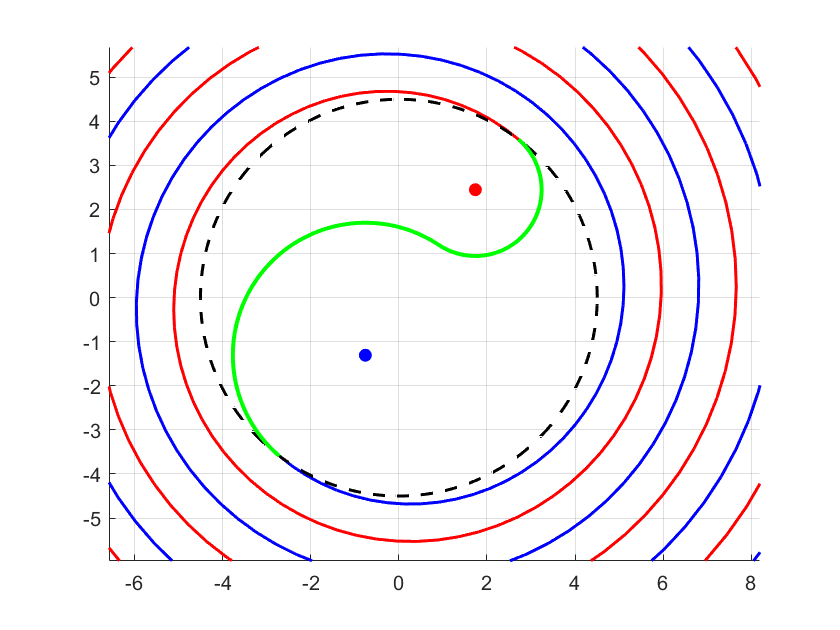
\includegraphics[width=0.7\linewidth]{drawing_5.4.1.2.png}
    \label{solving}
\end{figure}
\par
在该问题中,同样需要求出的是$P_1,P_2,P_3$坐标,以及向量$\overrightarrow{O_1 P_1}, \overrightarrow{O_1 P_3},\overrightarrow{O_2 P_2},\overrightarrow{O_2 P_3}$供下一小问求解使用。
\subsubsection{给定路径下龙头分时段运动状态分析}
\par
结合问题1和问题2,要求解所有把手的实时运动状态,问题的关键就在于求出龙头把手的实时位置坐标。一旦求出了龙头把手的实时坐标,就可以通过循环迭代依次从龙头把手开始遍历后续所有把手,
得到后续所有把手的位置坐标,而一旦求出了所有把手的位置坐标,通过求解当前时刻$t$之后一段微小时间$\delta t$后所有把手的位置状态,作差值并将$\delta t$内的平均速度近似为时刻$t$
时的瞬时速度,就可以得到所有把手实时速度关于时间$t$的函数。
下面我们着重来研究龙头把手在任意时刻的位置信息。
\par
根据题目要求,龙头把手刚刚到达$P_1$的时刻被重新记为$t_0=0$,设龙头把手刚刚离开第一段圆弧的时刻是$t_{n1}$,
刚刚离开第二段圆弧的时刻是$t_{n2}$,在这之后龙头就沿着盘出螺线逐渐盘出。
\par
根据刚才的分析,龙头盘入掉头盘出的过程可以分成四个阶段如下所列:
\begin{enumerate}
    \item \textbf{第一阶段:}$t<t_0$,龙头在盘入螺线上逐渐向中心盘入。
    \item \textbf{第二阶段:}$t_0 \leq t<t_{n1}$,龙头走出盘入螺线进入第一条圆弧线未进入第二条圆弧线。
    \item \textbf{第三阶段:}$t_{n1} \leq t< t_{n2}$,龙头出第一条圆弧线进入第二条圆弧线未进入盘出螺线。
    \item \textbf{第四阶段:}$t \geq  t_{n2}$,龙头出第二条圆弧线进入盘出螺线。
\end{enumerate}
\par
下面对四个阶段分别进行分析,从而得到龙头的实时位置坐标方程,从而可以进行仿真模拟分析。
\par
\textbf{第一阶段:}$t<t_0=0$时盘入螺线方程保持不变:
\begin{equation}
    C_1:r(\theta)=\frac{1.7\theta}{2 \pi}
\end{equation}
\par
仿照第一问,将运动时的切向速度近似成速度,从而得到微分方程:
\begin{equation}
    \omega=\frac{v(t)}{r(t)}=\frac{d \theta}{dt}
\end{equation}
\par
注意,本题的初始时间点$t=0$时,质点角位移初始值是$\theta_0$(已经在上一小节中解出)。
相比于问题1,这里需要更改定积分上下限,有:
\begin{equation}
    \int_{0}^{t} \frac{2 \pi}{1.7} \,dt=\int_{\theta_0}^{\theta} \theta \,d \theta  
\end{equation}
\par
考虑到$t<t_0$,故积分结果还有t的项前面需要添加负号,即:
\begin{equation}
    \theta(t)=\sqrt{\theta_0^2-\frac{2 \pi t}{1.7}}
\end{equation}
\par
通过平面投影得到其平面坐标:
\begin{align}
    \begin{cases}
        x_1(t)=1.7 \theta(t) \cos \theta(t)/2 \pi\\
        y_1(t)=1.7 \theta(t) \sin \theta(t)/2 \pi\\
    \end{cases}
\end{align}
\par
由于质点线速度恒为1m/s,因此龙头走完两段弧线分别要
\begin{align}
    \begin{cases}
        t_n1=\theta_1 r_1/v=\theta_1 r_1\\
        t_n2=(\theta_1 r_1+\theta_2 r_2) /v=\theta_1 r_1+\theta_2 r_2\\
    \end{cases}
\end{align}
\par
\textbf{第二阶段:}$t_0 \leq t<t_{n1}$,
龙头在第一段圆弧上。假设圆弧位于点$h_1$处,则弧线长及对应圆心角$\Delta \theta_1$分别是

\begin{align}
    \begin{cases}
        \overset{\LARGE{\frown}}{P_1 h_1}=vt=t\\
        \Delta \theta_1=\overset{\LARGE{\frown}}{P_1 b_1}/r_1=t/r_1\\
    \end{cases}
\end{align}
\par
因此$\overrightarrow{O_1  h_1}$是由$\overrightarrow{O_1  P_1}$顺时针旋转$\Delta \theta_1$
得到。根据顺时针坐标旋转公式,可以得到位置坐标关系:
\begin{align}
    \begin{cases}
        \overrightarrow{O_1  h_1}=
        \begin{bmatrix}
            \cos\Delta \theta_1 & \sin\Delta \theta_1 \\
            -\sin\Delta \theta_1 & \cos\Delta \theta_1
        \end{bmatrix}
        \cdot \overrightarrow{O_1  P_1}\\
        h_1=O_1+\overrightarrow{O_1  h_1}\\
        x_1(t)=h_{ix},y_1(t)=h_{1y}
    \end{cases}
\end{align}
\par
\textbf{第三阶段:}$t_{n1} \leq t< t_{n2}$,龙头在第二条圆弧线上,设某时刻龙头位于
$h_2$处。仿照上面的分析,显然有方程组:
\begin{align}
    \begin{cases}
        \overset{\LARGE{\frown}}{P_3 h_2} = v(t - t_{n1}) = t - t_{n1}, \\
        \Delta \theta_2 = \overset{\LARGE{\frown}}{P_3 h_2}/r_2 = t - t_{n1}/r_2, \\
        \overrightarrow{O_2 h_2} =
        \begin{bmatrix}
            \cos \Delta \theta_2 & -\sin \Delta \theta_2 \\
            \sin \Delta \theta_2 & \cos \Delta \theta_2
        \end{bmatrix}
        \cdot \overrightarrow{O_2 P_3}, \\
        h_2 = O_2 + \overrightarrow{O_2 h_2}, \\
        x_1(t) = h_{2x}, \quad y_1(t) = h_{2y}.
    \end{cases}
\end{align}
\par
\textbf{第四阶段:}$t \geq  t_{n2}$,龙头进入盘出螺线。
根据盘入螺线和盘出螺线的中心对称性质,可以求出相应盘入螺线上的点,再关于原点取中心对称。
设某时刻龙头位于离开盘出螺线前进$t-t_{n2}$时刻位于$h'$,根据$h$与$h'$的中心对称性可知,有:
\begin{align}
    \begin{cases}
        h'_x=x_1(t_n-t)\\
        h'_y=y_1(t_n-t)\\
        h_x=-h'_x=-x_1(t_n-t)\\
        h_y=-h'_y=-y_1(t_n-t)
    \end{cases}
\end{align}
\par
求解上述方程组:
\begin{align}
    \begin{cases}
        x_1(t)=-x_1(t_n-t)\\
        y_1(t)=-y_1(t_n-t)\\
    \end{cases}
\end{align}
\par
综上所述,龙头把手关于时间$t$的坐标$(x_1(t),y_1(t))$函数如下:
\begin{equation}
    \begin{aligned}
        & \begin{cases}
            x_1(t)=1.7 \theta(t) \cos \theta(t)/2 \pi & t<t_0\\
            x_1(t)=h_{ix} & t_0 \leq t<t_{n1} \\
            x_1(t) = h_{2x} & t_{n1} \leq t< t_{n2} \\
            x_1(t)=-x_1(t_n-t)  & t \geq  t_{n2} \\
        \end{cases}
        \quad
        \begin{cases}
            y_1(t)=1.7 \theta(t) \sin \theta(t)/2 \pi & t<t_0\\
            y_1(t)=h_{1y} & t_0 \leq t<t_{n1} \\
            y_1(t) = h_{2y} & t_{n1} \leq t< t_{n2} \\
            y_1(t)=-y_1(t_n-t) & t \geq  t_{n2} \\
        \end{cases}
    \end{aligned}
\end{equation}
\subsubsection{递推法求解任意时刻所有把手的运动状态}
\begin{figure}[hp]
    \caption{调头前后重要时刻图}
    \centering    
    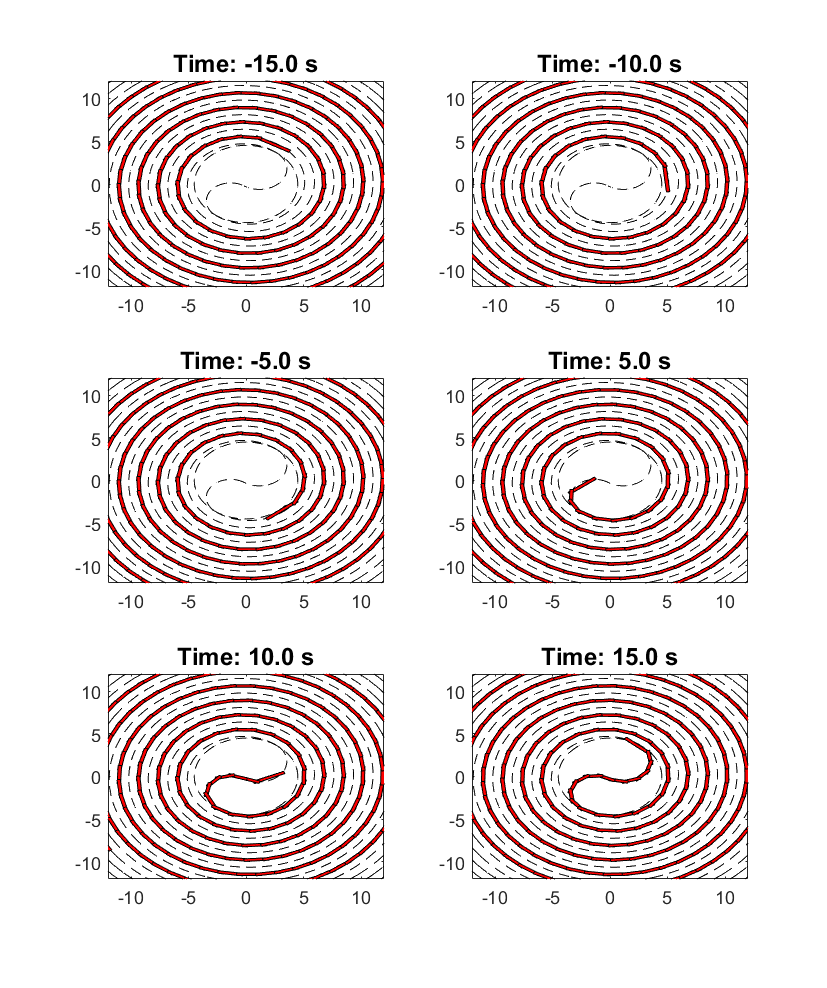
\includegraphics[width=0.79\linewidth]{drawing_5.4.4.2.png}
\end{figure}
正如问题1的思路,只要已知了龙头把手的位置状态,就可以通过一个循环遍历后续所有把手,得到在任意时刻下
所有把手的位置状态。对于这些位置状态,赋予时间$t$一个微小的扰动$\delta t$,用在$\delta t$内发生微小位移的平均速度来近似替代
在$t$的时刻的平均速度。
\par
与算法1(循环近似法求解下一把手的位置坐标)不同的是,对于下一个把手的计算,由于掉头半径的存在,前一把手和后一把手可能不再同一条曲线上,因此在迭代时
还需要对把手所处曲线的类型进行判断,下面我们介绍一种新算法4。如图16所示,算法4解决了在复杂路径下后续把手的分类计算问题,在通过代码实现的过程中,可以封装成一个函数体,嵌套至算法1中参加循环迭代过程。

\begin{figure}[h]
    \caption{算法流程图分析}
    \centering    
    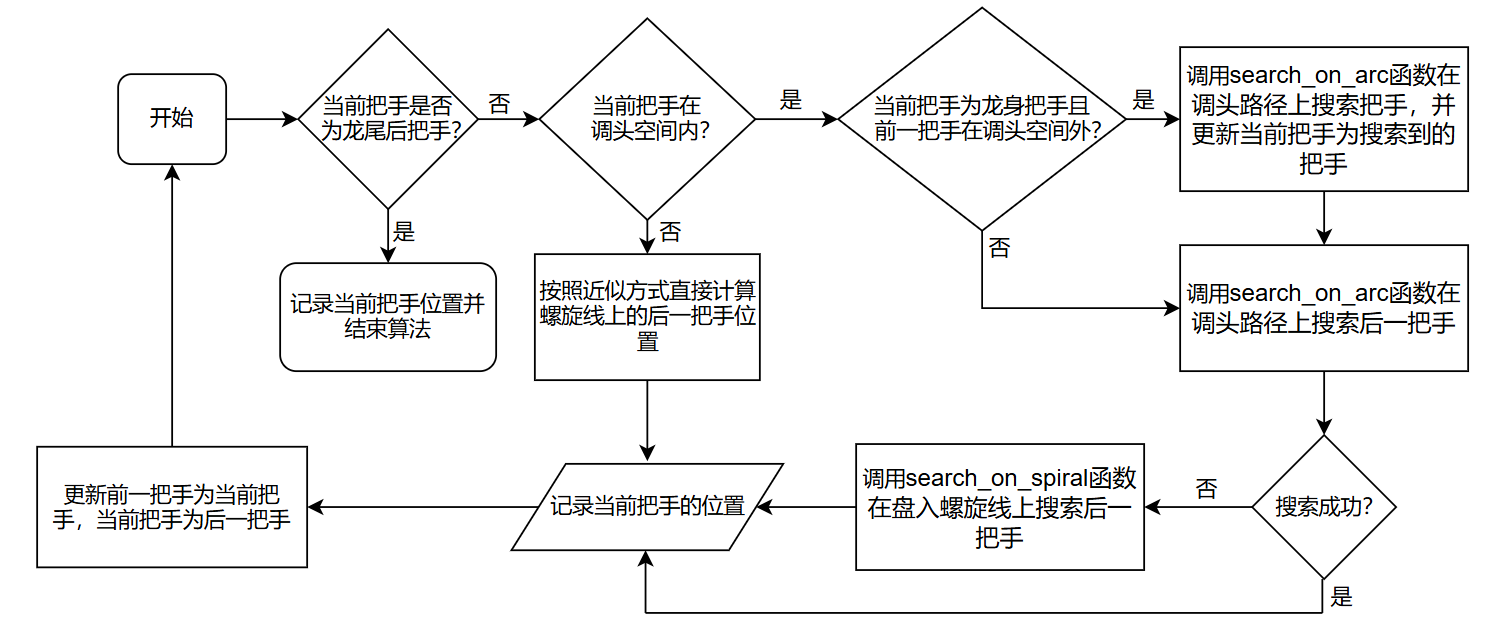
\includegraphics[width=0.97\linewidth]{drawing_5.4.4.1.png}
\end{figure}
\par
首先需要介绍算法4所需要的几个相关辅助函数:
\newline
\noindent
\textbf{位置判断函数1:}接受当前把手的位置坐标,计算其矢径长度并与掉头半径$R$进行比较从而判断当前把手是否在掉头区域内,返回一个布尔值。
是则传递并继续调用近似螺旋搜索函数,否则传递并调用$R$内搜索方向判断函数3。
\newline
\noindent
\textbf{近似螺旋搜索函数2:}对应图中函数search\_on\_spiral,它接受当前把手的坐标,通过近似螺旋法求解下一把手对应角位移大小,相应计算出其位置坐标。
\newline
\noindent
\textbf{R内搜索方向判断函数3:}对应图中函数search\_on\_arc,它接受当前把手i的坐标$(x_i,y_i)$,若把手i调头空间内部,可以肯定把手i一定在掉头区域中的两段圆弧上。
由于区域内有两段圆弧,时针方向不同。可以分别计算$(x_i,y_i)$与$(x_1,y_1)$和$(x_2,y_2)$的距离,比较与各自对应半径长的差值。若与圆$O_2$的差值
更大,则说明把手在圆$O_1$上,返回布尔值并传递给“圆弧内搜索函数4A”,反之传递给“圆弧内搜索函数4B”。如果把手i不在调头空间内部,则直接调用圆弧内搜索函数4A,从盘出螺旋线和调头空间的交点沿第二段圆弧进行搜索。
\newline
\noindent
\textbf{圆弧内搜索函数4A:}顺时针开始搜索第i+1个把手的位置,连接该把手与圆心$O_1$,取$\Delta \varphi $,从一个微小的步长开始递增$\Delta \varphi $,直至
两个把手的长度正好是$L$,然后使用圆的相关知识求解具体点坐标。
\newline
\noindent
\textbf{圆弧内搜索函数4B:}逆时针开始搜索第i+1个把手的位置,原理同上。
\par
有了以上五个函数,我们可以将相同功能的代码封装起来,只保留接口。这样也简化了该算法的流程。
\par
\textbf{算法4:复杂路径下后续把手的分类计算模型:}
\newline
\noindent
\textbf{输入:}上一轮循环中求得的各个龙头任意时刻的位置坐标。
\newline
\noindent
\textbf{输出:}“板凳龙”各个把手任意时刻的坐标(一旦坐标已知,就可以求出实时速度并作出模拟仿真动画)
\newline
\noindent
\textbf{S1:}从龙头把手出发,依次向后迭代循环。首先传入“位置判断函数1”,按照上面函数间的相互关系依次调用。
最终在
“位置判断函数1”,“圆弧内搜索函数4A”和“圆弧内搜索函数4B”这三个函数中停止并全部返回布尔正值。
\newline
\noindent
\textbf{S2:}判断当前把手是否为最后一个把手,如果是,则停止循环。
\par
在已知所有把手的运动状态后,不难对其进行实时过程仿真模拟,图15为调头前后重要时刻的模拟图,从中可以看出,根据我们的算法求出的位置极好地拟合了所有板凳龙的正确位置。

\subsection{\textbf{问题5}模型建立与求解}
问题五要求我们确定舞龙队沿问题四设定的路径行进时,龙头的最大行进速度,使得舞龙队各把手的速度均不超过2m/s。因此,这个问题的本质是一个约束优化问题,我们需要在保证所有板凳速度不超过限制的前提下,最大化龙头的行进速度。
\par
首先,我们需要明确问题的约束条件。龙头的行进速度是我们的优化目标,而所有板凳(包括龙头)的速度不超过2m/s是我们的约束条件。这意味着我们需要建立一个模型,能够根据龙头的行进速度计算出板凳龙所有部分的速度。其次,我们需要考虑路径的几何特性如何影响板凳龙的运动。问题四中设定的路径是一个S形曲线,由两段圆弧组成。在这种曲线路径上,即使龙头保持恒定速度,其他部分的速度也会因为路径曲率的变化而发生变化。我们需要仔细分析这种关系,以确保在整个运动过程中所有部分的速度都不会超过限制。
再者,我们需要考虑板凳龙的结构特性。板凳之间的连接方式和相对位置关系会影响速度的传递。特别是,由于板凳龙是一个长链状结构,靠近尾部的板凳会经历更大的速度变化,这成为限制最大速度的关键因素。
\par
在问题4的基础上,我们将v作为变量,将问题4中求出的函数转化为关于t,v的函数。

\subsubsection{\textbf{问题5}模型的分析与求解}

\par
\textbf{算法5:迭代求速度:}
\newline
\noindent
\textbf{S1:}初始化参数:记时间步长为1秒,终止时间为100秒,确保结束时间足够大而不会遗漏结果。
\noindent
\newline
\textbf{S2:}进入第一轮循环,每一个循环节将会对应一个时刻。调用之前问题求得的函数来计算每时刻所有把手的位置。具体来说,先计算龙头前把手的位置,再从龙头开始依次计算每个把手的位置。
\newline
\noindent
\textbf{S3:}第一轮循环结束,即将进入第二轮循环。每一个循环节对应一个板凳的判断过程,根据当前把手是第一个把手还是后续把手确定距离,判断当前把手是否在调头空间内。若不在当前空间内,按照近似方式计算下一个把手。
\newline
\noindent
\textbf{S4:}按照第一段圆弧、第二段圆弧以及盘出对把手的运动进行分类和筛选。调头过程中,搜寻在螺旋线上的下一个点。设定一个小的角度步长,如果距离达到了目标距离,则返回当前螺旋线上的点。
\newline
\noindent
\textbf{S5:} 定义初始龙头速度和步长,龙头速度初始为1m/s。 开始迭代速度,从1m/s逐步增加,获取所有把手的位置信息,检查是否有把手速度超过了2m/s,若没有,则继续循环;若出现这种情况,则跳出循环,并且输出此时的龙头速度,即最终的最大速度。
\par
问题4导出的函数:
\begin{equation}
    \textbf{X(t)}=
    \begin{bmatrix}
    x_1(t)\\
    x_3(t)\\
    \vdots\\
    x_n(t)\\
    \end{bmatrix}
\end{equation}
\begin{equation}
    \textbf{Y(t)}=
    \begin{bmatrix}
    y_1(t)\\
    y_3(t)\\
    \vdots\\
    y_n(t)\\
    \end{bmatrix}
\end{equation}
\par
上述两个函数是关于t,v的函数,即可以写成:
\begin{equation}
    \textbf{X}(t)= \textbf{X}(t,v_{head})
\end{equation}
\begin{equation}
    \textbf{Y}(t) = \textbf{Y}(t,v_{head})
\end{equation}
\par
同理可得:
\begin{equation}
    \textbf{v}(t) = v(t,v_{head})
\end{equation}
\par
由问题4所导出的结果可知,当$v_{head}$=1m/s时,所有把手在[-100,100]这一区间上的运动速度均不超过2m/s,因此,我们不妨选取$v_{head}$=1m/s为起点,以$dv=0.01m/s$为步长不断增加。直到某一点$v(t,v_{head}) >2m/s$时,有最大值$v=v_{head}-dv$。经过多次迭代,我们计算出的结果为1.10m/s。
\begin{figure}[htbp]
    \caption{龙身最大速度随龙头最大速度的变化曲线}
    \centering    
    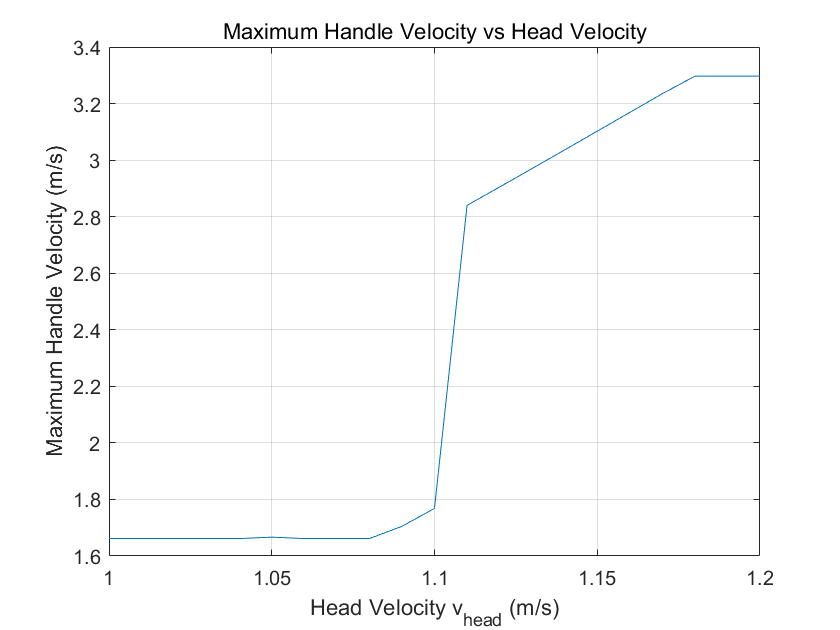
\includegraphics[width=0.7\linewidth]{5.5.1.png}
\end{figure}

\subsubsection{问题5结果的验证与处理}
我们结合物理学知识,利用MATLAB进行模拟仿真,绘制出龙身最大速度与龙头最大速度之间的关系曲线,如图17所见。可以看出,随着龙头最大速度的增加,龙身的最大速度也不断增加,这是符合真实的物理情景的。值得注意的是,当龙头最大速度达到1.1m/s时,龙身最大速度立刻发生了突跃,迅速突破2m/s的上限。因此,我们确定龙头的最大速度为1.1m/s.

\begin{figure}[htbp]
    \caption{龙头速度最大时,七节龙身的速度变化曲线}
    \centering    
    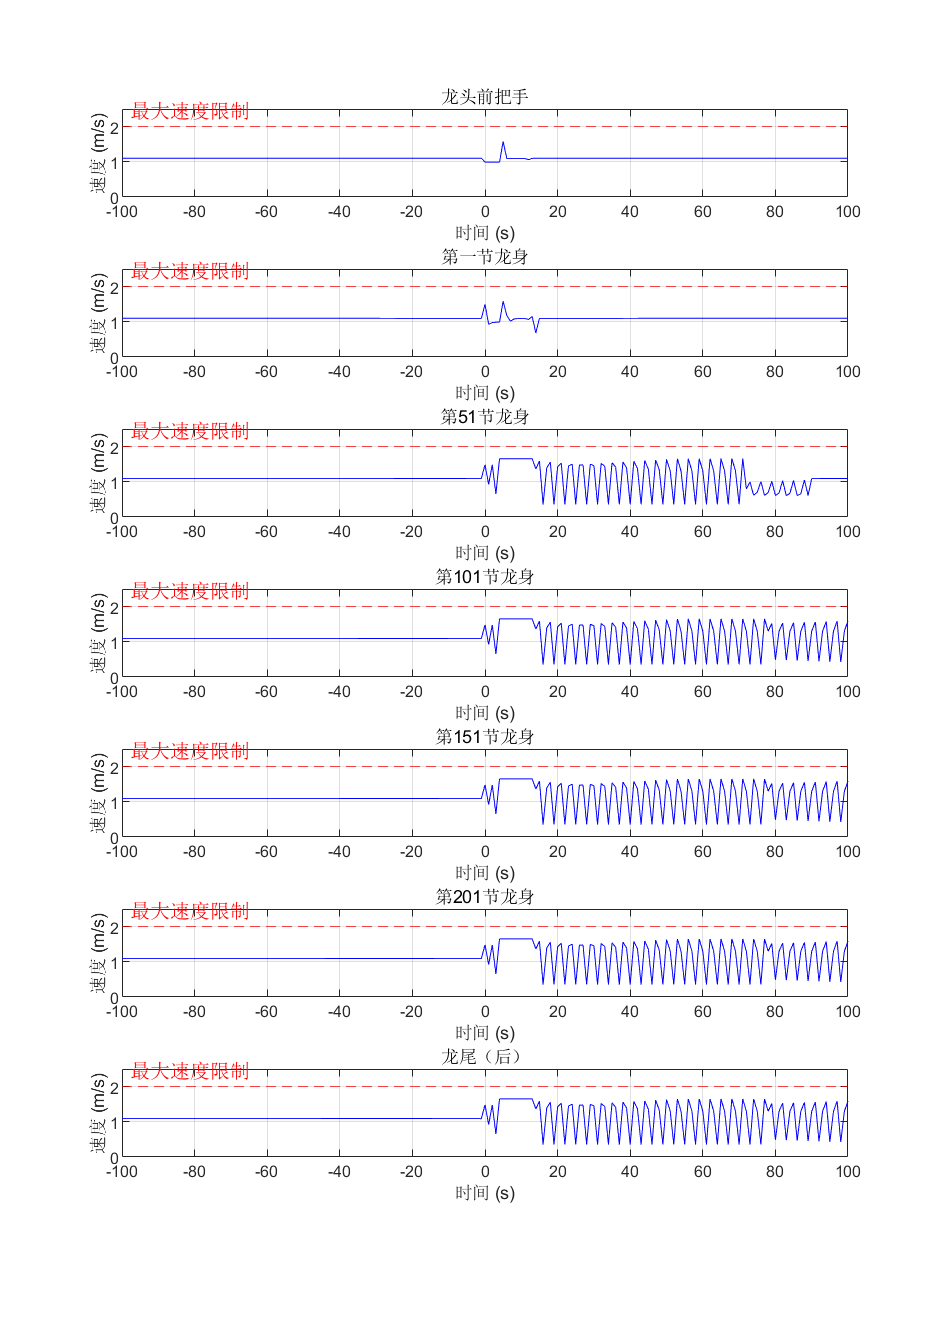
\includegraphics[width=0.7\linewidth]{5.5.3.png}
\end{figure}

确定龙头的最大行进速度后,我们选取了七节龙身,并研究其速度变化特征,如图18所示。可以发现,在0s(初始时刻即将运动)时,七节龙身的速度均约为1m/s,这与问题1和问题2的给定条件不谋而合。当龙头达到最大速度后,七节龙身都突然获得了一定的速度。不同之处在于,龙头前把手与第一节龙身的速度很快便回到1m/s附近,然后不再变动;第51、101、151、201节龙身的速度则开始以1m/s为准线上下振荡起来。由之前的分析不难联想到,这与板凳之间的连锁运动有着密不可分的关系。




\section{模型评估}
\subsection{模型误差及其校正}
\subsubsection{问题1相关误差与修正方法}
\begin{enumerate}
    \item 由于“板凳龙”的把手沿着螺旋线运动,而螺旋线并不是一个严格的圆弧,这就导致了其线速度和螺旋矢径之间的夹角并不是一个严格的直角,必然存在几度或分秒级别的误差。我们将这样的螺旋运动在各个时刻下的状态与其在同样半径的圆弧运动作了一步近似。近似之后,我们便可以忽略径向速度,并将圆周的切向速度等效为螺旋运动的线速度。
    \item 我们使用余弦法求后续龙身把手位置,得到的迭代方程属于超越方程,无法求出其解析解。因此我们只能通过尽可能优化的近似手段来求出近似解。我们令$\Delta \theta$ 从0开始逐渐增加步长,遍历到L的全过程。随着迭代次数的增加,计算更外围的把手时,其误差更大,而当时刻$t$逐渐增加后,随着把手向内运动,其精度会越来越高。
    \item 除了余弦法之外,我们另外还使用了近似圆弧法求解后续龙身把手位置,即处理半径较大的螺线时,我们可以将其等效为圆弧处理。这样做的合理性是,转过一圈时,半径衰减的幅度所对应的数量级远远小于半径所对应的数量级,误差约为小数点后四位,精度较好,并且通过近似圆弧法相较于余弦法更容易被计算机实现。
    \item 我们使用差分法来求解把手的速度。由于无法对全过程进行连续的模拟仿真,我们只能取多个相隔很近、分立的值。我们重新设置一个关于时刻t新的步长$\delta t$=0.0001。用从这一时刻开始的微小时间内的平均速度近似代替在该时刻的瞬时速度。这是一种非常经典却又精度较高的近似方法。
\end{enumerate}
\subsubsection{问题2,3相关误差与修正方法}
\begin{enumerate}
    \item 问题2是基于问题1的仿真模拟所给出的实时数据来解决的,因此问题2的求解在先天上便存在有问题1带来的全部问题。例如由于龙头把手的坐标是由切向速度近似成线速度得到的,而这一数据又在后面作为循环头,开启若干轮遍历,故一开始的误差会随着时间逐渐累积。
    \item 问题2需要求解出龙头后续18个板凳的4个边界点的坐标,由于计算这些坐标值需要大量中间量,例如计算方向向量,单位方向向量,单位切线向量,这个计算过程会导致其中间变量的误差逐渐累积到最终数值中。
    \item 受限于循环迭代操作中时间步长的大小影响,永远没有办法得到精确的碰撞时刻,因为进行求解的只能是离散的时间状态,所以距离真实过程中连续的物体运动过程始终有一定差值。想要解决这个问题,只需要再计算机允许求解的复杂度的情况下,不断缩小其步长,逼近连续过程。
    \end{enumerate}
\subsubsection{问题4,5相关误差与修正方法}
\begin{enumerate}
    \item 问题4在求解掉头最短路径一问误差值较小,原因在于我们没有对该非线性规划问题的任何数值或者约束条件作任何近似处理,在传入计算机后,其误差仅仅来自于编译器求解的误差,一般来说matlab求解器精度较高,可以达到小数点后六位。
    \item 问题4第二小问误差相当更大了,与1类似,这种根据龙头节点开始循环得到的位置矩阵在经过多轮循环后误差会逐渐累积,同时时间由于取值离散化的原因导致精确时间测不准。这些误差和问题2类似。
    \item 在这里,“板凳龙”是在由4条曲线拼接而成的曲线内运动,在计算相邻节点运动状态时,还需要考虑一个节点在圆弧内,一个节点在圆弧外,在涉及这样的一轮循环后,需要调用更多的函数体进行求解。同时,对于横跨两段曲线的求解过程,使用的近似螺旋在这里的计算误差更大误差更大。
    \item 在最后求解实时速度时,在选取一段微小的时间时发生了较大的误差。在计算机编译时,若选取小于0.5的微小时间,会使得计算出的某些相邻时间内数值发生突变跃升至几千米每秒,这显然是不可能得,因此,为了同时兼顾数值的准确性与可计算型,最终取得一段微小的时间长度为1m/s。
    \end{enumerate}
\subsection{模型优缺点及推广}
\begin{enumerate}
    \item 优点:模型被极大地简化了,问题1使用近似螺旋法,将螺旋线等价为圆弧处理。在计算速度时不去探究速度精准的解析表达式,而是直接用一段微小时间内的平均速度进行近似。问题本身是一个连续型的仿真模拟问题,我们取离散的时刻值,不断缩小时间步长来趋近于连续。最后一问将问题逐步分解为若干个函数块,彼此之间相互调用,简单方便。
    \item 缺点:误差较大,第一轮近似螺旋法求得的龙头坐标本身存在误差,这些误差经过一步步循环逐步累积。无法得到精确的位置坐标和速度的解析表达式,而根据物理原理,确定的过程具有确定的解,理论上其确定的解析表达式一定存在,而这里只研究数值解。不是连续类型模型,与实际有所差距。
    \item 启发:交通运输过程中的车辆运动问题,更精确地认识车流量、碰撞的物理意义,从而减少交通事故的发生。对自然界中某些生物现象的研究,比如昆虫的成群移动等,推进人们对于自然界的认识。对中国传统文化的弘扬,从数学等专业角度给出了“板凳龙”舞动更加美丽的策略。
\end{enumerate}



\newpage
\section{附录}




\end{document} 